\documentclass[]{article}
\usepackage{lmodern}
\usepackage{amssymb,amsmath}
\usepackage{ifxetex,ifluatex}
\usepackage{fixltx2e} % provides \textsubscript
\ifnum 0\ifxetex 1\fi\ifluatex 1\fi=0 % if pdftex
  \usepackage[T1]{fontenc}
  \usepackage[utf8]{inputenc}
\else % if luatex or xelatex
  \ifxetex
    \usepackage{mathspec}
  \else
    \usepackage{fontspec}
  \fi
  \defaultfontfeatures{Ligatures=TeX,Scale=MatchLowercase}
\fi
% use upquote if available, for straight quotes in verbatim environments
\IfFileExists{upquote.sty}{\usepackage{upquote}}{}
% use microtype if available
\IfFileExists{microtype.sty}{%
\usepackage{microtype}
\UseMicrotypeSet[protrusion]{basicmath} % disable protrusion for tt fonts
}{}
\usepackage[margin=1in]{geometry}
\usepackage{hyperref}
\hypersetup{unicode=true,
            pdftitle={test},
            pdfborder={0 0 0},
            breaklinks=true}
\urlstyle{same}  % don't use monospace font for urls
\usepackage{color}
\usepackage{fancyvrb}
\newcommand{\VerbBar}{|}
\newcommand{\VERB}{\Verb[commandchars=\\\{\}]}
\DefineVerbatimEnvironment{Highlighting}{Verbatim}{commandchars=\\\{\}}
% Add ',fontsize=\small' for more characters per line
\usepackage{framed}
\definecolor{shadecolor}{RGB}{248,248,248}
\newenvironment{Shaded}{\begin{snugshade}}{\end{snugshade}}
\newcommand{\KeywordTok}[1]{\textcolor[rgb]{0.13,0.29,0.53}{\textbf{#1}}}
\newcommand{\DataTypeTok}[1]{\textcolor[rgb]{0.13,0.29,0.53}{#1}}
\newcommand{\DecValTok}[1]{\textcolor[rgb]{0.00,0.00,0.81}{#1}}
\newcommand{\BaseNTok}[1]{\textcolor[rgb]{0.00,0.00,0.81}{#1}}
\newcommand{\FloatTok}[1]{\textcolor[rgb]{0.00,0.00,0.81}{#1}}
\newcommand{\ConstantTok}[1]{\textcolor[rgb]{0.00,0.00,0.00}{#1}}
\newcommand{\CharTok}[1]{\textcolor[rgb]{0.31,0.60,0.02}{#1}}
\newcommand{\SpecialCharTok}[1]{\textcolor[rgb]{0.00,0.00,0.00}{#1}}
\newcommand{\StringTok}[1]{\textcolor[rgb]{0.31,0.60,0.02}{#1}}
\newcommand{\VerbatimStringTok}[1]{\textcolor[rgb]{0.31,0.60,0.02}{#1}}
\newcommand{\SpecialStringTok}[1]{\textcolor[rgb]{0.31,0.60,0.02}{#1}}
\newcommand{\ImportTok}[1]{#1}
\newcommand{\CommentTok}[1]{\textcolor[rgb]{0.56,0.35,0.01}{\textit{#1}}}
\newcommand{\DocumentationTok}[1]{\textcolor[rgb]{0.56,0.35,0.01}{\textbf{\textit{#1}}}}
\newcommand{\AnnotationTok}[1]{\textcolor[rgb]{0.56,0.35,0.01}{\textbf{\textit{#1}}}}
\newcommand{\CommentVarTok}[1]{\textcolor[rgb]{0.56,0.35,0.01}{\textbf{\textit{#1}}}}
\newcommand{\OtherTok}[1]{\textcolor[rgb]{0.56,0.35,0.01}{#1}}
\newcommand{\FunctionTok}[1]{\textcolor[rgb]{0.00,0.00,0.00}{#1}}
\newcommand{\VariableTok}[1]{\textcolor[rgb]{0.00,0.00,0.00}{#1}}
\newcommand{\ControlFlowTok}[1]{\textcolor[rgb]{0.13,0.29,0.53}{\textbf{#1}}}
\newcommand{\OperatorTok}[1]{\textcolor[rgb]{0.81,0.36,0.00}{\textbf{#1}}}
\newcommand{\BuiltInTok}[1]{#1}
\newcommand{\ExtensionTok}[1]{#1}
\newcommand{\PreprocessorTok}[1]{\textcolor[rgb]{0.56,0.35,0.01}{\textit{#1}}}
\newcommand{\AttributeTok}[1]{\textcolor[rgb]{0.77,0.63,0.00}{#1}}
\newcommand{\RegionMarkerTok}[1]{#1}
\newcommand{\InformationTok}[1]{\textcolor[rgb]{0.56,0.35,0.01}{\textbf{\textit{#1}}}}
\newcommand{\WarningTok}[1]{\textcolor[rgb]{0.56,0.35,0.01}{\textbf{\textit{#1}}}}
\newcommand{\AlertTok}[1]{\textcolor[rgb]{0.94,0.16,0.16}{#1}}
\newcommand{\ErrorTok}[1]{\textcolor[rgb]{0.64,0.00,0.00}{\textbf{#1}}}
\newcommand{\NormalTok}[1]{#1}
\usepackage{longtable,booktabs}
\usepackage{graphicx,grffile}
\makeatletter
\def\maxwidth{\ifdim\Gin@nat@width>\linewidth\linewidth\else\Gin@nat@width\fi}
\def\maxheight{\ifdim\Gin@nat@height>\textheight\textheight\else\Gin@nat@height\fi}
\makeatother
% Scale images if necessary, so that they will not overflow the page
% margins by default, and it is still possible to overwrite the defaults
% using explicit options in \includegraphics[width, height, ...]{}
\setkeys{Gin}{width=\maxwidth,height=\maxheight,keepaspectratio}
\IfFileExists{parskip.sty}{%
\usepackage{parskip}
}{% else
\setlength{\parindent}{0pt}
\setlength{\parskip}{6pt plus 2pt minus 1pt}
}
\setlength{\emergencystretch}{3em}  % prevent overfull lines
\providecommand{\tightlist}{%
  \setlength{\itemsep}{0pt}\setlength{\parskip}{0pt}}
\setcounter{secnumdepth}{5}
% Redefines (sub)paragraphs to behave more like sections
\ifx\paragraph\undefined\else
\let\oldparagraph\paragraph
\renewcommand{\paragraph}[1]{\oldparagraph{#1}\mbox{}}
\fi
\ifx\subparagraph\undefined\else
\let\oldsubparagraph\subparagraph
\renewcommand{\subparagraph}[1]{\oldsubparagraph{#1}\mbox{}}
\fi

%%% Use protect on footnotes to avoid problems with footnotes in titles
\let\rmarkdownfootnote\footnote%
\def\footnote{\protect\rmarkdownfootnote}

%%% Change title format to be more compact
\usepackage{titling}

% Create subtitle command for use in maketitle
\newcommand{\subtitle}[1]{
  \posttitle{
    \begin{center}\large#1\end{center}
    }
}

\setlength{\droptitle}{-2em}
  \title{test}
  \pretitle{\vspace{\droptitle}\centering\huge}
  \posttitle{\par}
  \author{}
  \preauthor{}\postauthor{}
  \predate{\centering\large\emph}
  \postdate{\par}
  \date{16 March, 2018}

\usepackage{bbm} 
\newcommand{\D}{\text{d}}
\newcommand{\indicator}{\mathbbm{1}}
\newcommand{\hamm}{d_h}
\newcommand{\symhamm}{d_{sh}}
\newcommand{\hz}{\text{Hz}}
\newcommand{\tr}{\text{tr}}
\newcommand{\Iext}{{I_e/A}}
\newcommand\gvn[1][]{\:#1\vert\:}
\usepackage{afterpage}
\usepackage{fancyvrb}
\usepackage{longtable}
\usepackage{booktabs} 
\usepackage{placeins}

\usepackage{amsthm}
\newtheorem{theorem}{Theorem}[section]
\newtheorem{lemma}{Lemma}[section]
\theoremstyle{definition}
\newtheorem{definition}{Definition}[section]
\newtheorem{corollary}{Corollary}[section]
\newtheorem{proposition}{Proposition}[section]
\theoremstyle{definition}
\newtheorem{example}{Example}[section]
\theoremstyle{definition}
\newtheorem{exercise}{Exercise}[section]
\theoremstyle{remark}
\newtheorem*{remark}{Remark}
\newtheorem*{solution}{Solution}
\begin{document}
\maketitle

{
\setcounter{tocdepth}{4}
\tableofcontents
}
\section{Main}\label{main}

\subsection{Finding priors for the beta
distribution}\label{finding-priors-for-the-beta-distribution}

Beta distribution is the natural prior for a binomial/bernoulli
distribution. Considering distribution of a binomial variable
\(X\gvn\theta\sim Binom(\theta)\), in order to make its marginalisd
distribution \(P(X) = \int P(X\gvn\theta)P(\theta).d\theta\)
analytically tractable, one of the choice is to assume
\(\theta\sim Beta(M,\alpha)\), so that:

\[
\begin{aligned}
P(\theta) &=\frac{x^{\alpha - 1}(1-x)^{M-\alpha-1}}{B(\alpha,M-\alpha)}
\\
E(\theta) &={\alpha\over M }
\end{aligned}
\]

\subsubsection{Constraint 1:}\label{constraint-1}

\[
\begin{aligned}
P(\theta\le 0.25) = P(\theta\ge 0.75) =  0.05 \\
P(\theta\le 0.75)=0.95
\end{aligned}
\]

Fitted result: \(\theta\sim\) Beta(4.933, 4.932 )

\subsubsection{Constraint 2}\label{constraint-2}

\[
\begin{aligned}
\text{argmax}_\theta(P(\theta))=0.4 \\
P(\theta\le 0.3) = 0.1
\end{aligned}
\]

Fitted result: \(\theta\sim\) Beta(13.863, 20.295 )

\begin{figure}
\centering
\includegraphics{net1_fg368_files/figure-latex/constrained-beta-1.pdf}
\caption{\label{fig:constrained-beta}The shape of the beta distribution
constrianed under the respective conditions. Left: Constraint 1. Right:
Constraint 2. (green: PDF, black: CDF)}
\end{figure}

\begin{figure}
\centering
\includegraphics{net1_fg368_files/figure-latex/bayes-1.pdf}
\caption{\label{fig:bayes}Inference of posterior distribution on parameter
\(\theta\) given mutatble sequence: 011100101101}
\end{figure}

\subsubsection{\texorpdfstring{Basics for Bayesian inference
\label{sec:bayes-basics}}{Basics for Bayesian inference }}\label{basics-for-bayesian-inference}

\[
\begin{aligned}
\text{likelihood}&: f(\theta) = P(x \gvn \theta) \\
\text{prior}&: f(\theta) = P(\theta) \\
\text{posterior}&: f(\theta)  = P(\theta \gvn x) = \frac{  P(x\gvn \theta) P(\theta)  }{P(x) } \\
\text{marginal likelihood} &: P(x) =  \int P(x\gvn \theta) P(\theta).d\theta
\end{aligned}
\]

The observed toss sequence is: 011100101101

Assume each coin toss is independent from each other, the likelihood of
an observed sequence is only dependent on the total number of heads and
not the sequence it occurred in. Denoting the coin toss as a sequence
\(\{x_i\}\) where \(x_i \in \{0,1\}\), we have

\[
\begin{aligned}
\text{\#head} = \indicator\{x_i=1\} \\
\text{\#head} \sim Binom(|\{x_i\}|,\theta)
\end{aligned}
\] Combining with the prior \(\theta\sim\) Beta(13.863, 20.295 ), I
calculated the marginal likelihood numerically to be \(P(x)=\) 0.11 and
derived the posterior distribution accordingly (see figure
\ref{fig:bayes}). MLE is obtained at \(\hat{\theta}=\) 0.45

\subsection{Inferring a three variable Bayesian
network}\label{inferring-a-three-variable-bayesian-network}

I reparametrise the joint probability of the graph by replacing the
conditional probability \(P(child|parent)\) to be the quotient of two
joint distirbution \(\frac{P(child,parent)}{P(parent)}\). Because
\(P(child|parent)\) enters the marginalised likelihood as a
Beta-Binomial probability, \(P(parent)\) enters the term as a
Drichlet-Multinomial probability:

\[
P(x_k)={\frac {\left(n!\right)\Gamma \left(\sum \alpha _{k}\right)}{\Gamma \left(n+\sum \alpha _{k}\right)}}\prod _{k=1}^{K}{\frac {\Gamma (x_{k}+\alpha _{k})}{\left(x_{k}!\right)\Gamma (\alpha _{k})}}
\] where \(\sum{x_k}=N\) is the partition of sample into k categories,
\(\alpha_k\) is the imaginary sample size for each category (also known
as prior concentration). This formulation has the advantage of easier
coding.

To be consistent with bnlearn and deal, I did discared the multinomial
terms in the calculation, leading to

\[
P(x_k)={\frac {\Gamma \left(\sum \alpha _{k}\right)}{\Gamma \left(n+\sum \alpha _{k}\right)}}\prod _{k=1}^{K}{\frac {\Gamma (x_{k}+\alpha _{k})}{\Gamma (\alpha _{k})}}
\]

\subsection{Number of Bayesian
networks:}\label{number-of-bayesian-networks}

A V-variable network has \(V(V-1)/2\) bivariate interaction (edges),
each interaction can have 3 possible status (A-\textgreater{}B,
A\textless{}-B, A B). Hence altogether there are \(n(V) = 3^{V(V-1)/2}\)
possible networks. For \(V=3\),\(n(3)=27\)

However, for this exerecise, the serach space is restircted to the graph
set \(G=\) \{no-edge, A-C only, A-C and B-C\}.

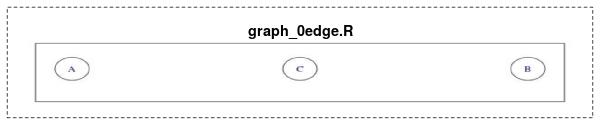
\includegraphics{graph_0edge.jpg} 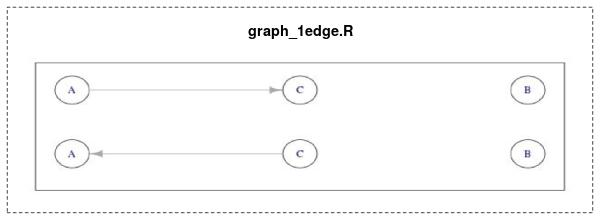
\includegraphics{graph_1edge.jpg}

\begin{figure}
\centering
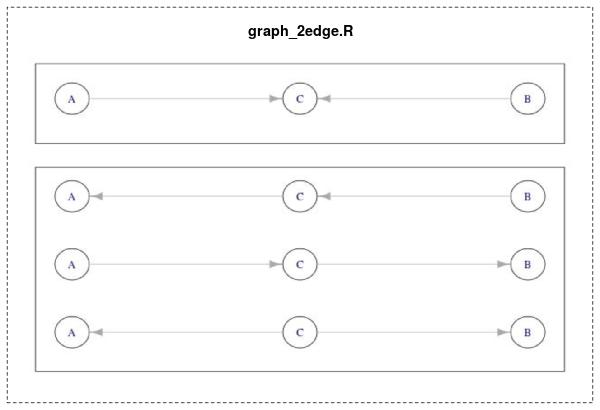
\includegraphics[height=0.50000\textwidth]{graph_2edge.jpg}
\caption{Graph with two edges but not A-B}
\end{figure}

\begin{figure}
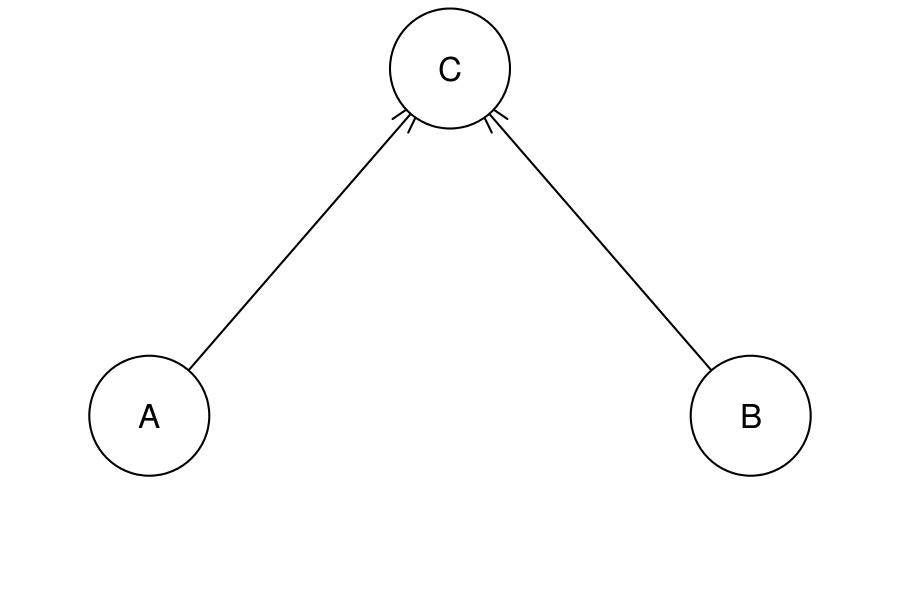
\includegraphics[width=0.45\textwidth]{pcalgo_dat1.png}
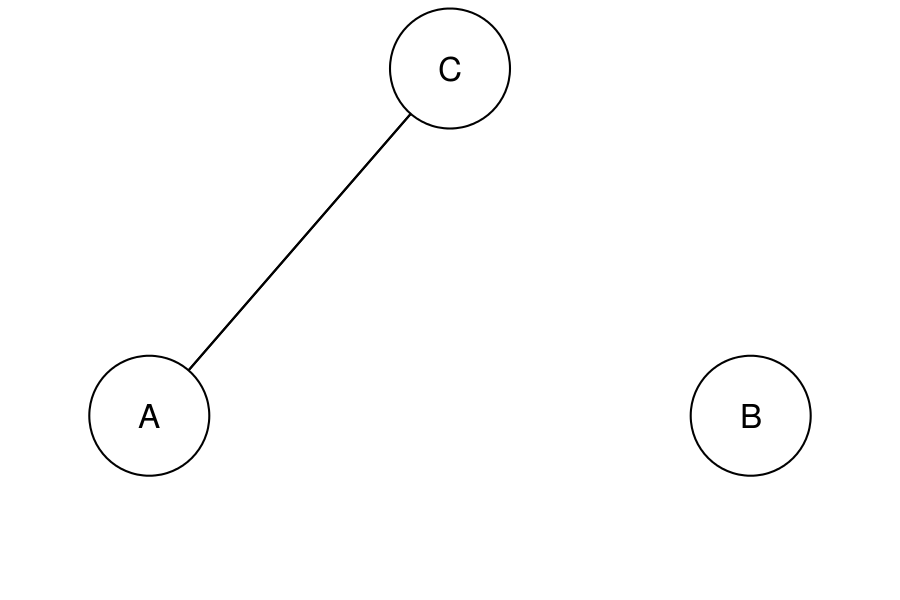
\includegraphics[width=0.45\textwidth]{pcalgo_dat2.png}
\caption{ \label{fig:pc-best}Best networks inferred using "bnlearn::pc.stable". Left: Dataset1. Right: Dataset2}
\end{figure}

\iffalse
\includegraphics[page=1,width=\paperwidth]{popgen_eqn_p3.pdf} \fi

\subsubsection{Comment on the likelihood-equivalent
prior}\label{comment-on-the-likelihood-equivalent-prior}

The likelihood-equivalent prior is set so that the imaginary sample size
decreases as data is stratified by more variables. For example, if
\(P(A=1) \sim Beta(\eta(A_0),\eta(A_1))\), then the imaginary sample
size for (A=1) is \(\eta(A_1)=2\). Hence if we then ask for
\(P(B=1\gvn A=1)\sim Beta(\eta(B_0A_1),\eta(B_1A_1))\), the imaginary
\(\eta\)'s must add up to the imageinary sample size of the condition
\(\gvn A=1\), (aka \(\eta(B_0A_1)+\eta(B_1A_1)=\eta(A_1)=2\)). Assuming
two events are equally probable gives \(\eta(B_0A_1)=\eta(B_1A_1)=1\).
For 3 variable, we can deduce \(8\eta(ABC)=4\eta(AB)=2\eta(A)=\eta(0)\),
setting \(\eta(ABC)=1\) gives
\(\eta(ABC)=1,\eta(AB)=2,\eta(A)=4,\eta(0)=8\), corresponding to
different levels of stratification.

If a likelihood-preserving prior is used, then it is only the
correlation structure that determines the relative feasibility of
different graphs. Consider the 1-edge and 0-edge examples, the 0-edge
example asserts \(P(A\gvn C=0)=P(A\gvn C=1)=P(A)\), whereas the 1-edge
example implies \(P(A\gvn C=0)\neq P(A\gvn C=1)\), allowing an
additional degree of freedom. The striking fact is that this additional
DOF does not necessarily leads to a better model, in constrast to
conventional mixture models where additional components always reduce
likelihood. One of the reason is that the partiaion of
\((A_0)=(A_0C_0)+(A_0C_1)\) is not arbitratry, but the general case is
still confusing. A possible intution is that the additional DOF project
the paramteric space to a higher dimension where the likelihood function
overlaps less with the prior distribution.

\subsubsection{Drawbacks of binary bayesian
networks}\label{drawbacks-of-binary-bayesian-networks}

If there are hidden latent variables in the bayes net, for example where
the common parent of A and B (which is C) is conceived from the
observers, then one will have to consider a graph with hidden variable
in order to explain the data. In other words, a graphical prior needs to
accommodate additional nodes to explain such data. Even though this is
the case, it will be hard to express the case where n(A\_0)=n(B\_0)

\subsubsection{Effect of imaginary sample
size}\label{effect-of-imaginary-sample-size}

Here we consider two imaginary sample sizes \(\eta(0)=8\) and
\(\eta(0)=1\). A higher \(\eta\) indicates a sharper distribution of
binomial probability \(\theta\) (Setting \(\eta(0)=1\) implies
\(\eta(ABC)=0.125,\eta(AB)=0.25,\eta(A)=0.5,\eta(0)=1\))

The corresponding likelihood are calculated for both datasets (dat1 and
dat2, see table \ref{tab:likelihood}).

\begin{itemize}
\item
  For dat1, the chain network (A-B-C) is the best at ISS=1, the A-B..C
  network is the best at ISS=8.
\item
  For dat2, the chain network (A-B-C) is the best for ISS=1 and ISS=8
\end{itemize}

The prediction made by pc.stable is somewhat different (figure
\ref{fig:pc-best})

\begin{figure}
\centering
\includegraphics{net1_fg368_files/figure-latex/c-gvn-a-idep-1.pdf}
\caption{\label{fig:c-gvn-a-idep}P(C\textbar{}A)=P(C) according to the
0-edge graph, Left: P(C\textbar{}A=0). Right: P(C\textbar{}A=1)}
\end{figure}

\begin{figure}
\centering
\includegraphics{net1_fg368_files/figure-latex/c-gvn-a-1.pdf}
\caption{\label{fig:c-gvn-a}P(C\textbar{}A) needs to be stratified according
to the 1-edge graph, Left: P(C\textbar{}A=0). Right: P(C\textbar{}A=1)}
\end{figure}

\subsubsection{Plot posteiror for P(C\textbar{}A) in different
models}\label{plot-posteiror-for-pca-in-different-models}

Here I visulise the posterior distribution using dataset 1 only. In
order to show how different graphical models lead to different
likelihood, I chose to contrast P(C\textbar{}A) between
\text{[A][B][C]}(0-edge model) and \text{[A][B][C|A]} (1-edge model)

In 0-edge model, \(P(C|A)=P(C)\) and the distribution is indifferent for
\(A=0\) and \(A=1\) (figure \ref{fig:c-gvn-a-idep}). The term enters
likelihood function as a beta-binomial.

In contrast, the 1-edge model prescribes that \(P(A,C)\neq P(A)P(C)\),
and two separate distribution must be considered for \(P(C|A)\) (figure
\ref{fig:c-gvn-a}). The \(\prod_{C,A} P(C|A)\) term factors out to be
\(\prod_{C|A=0} P(C|A=0)\prod_{C|A=0} P(C|A=1)\), as the product of two
beta-binomial with independent probability but the same prior. It would
be interesting to explore the precise condition under which the factored
likelihood exceeds the original single beta-binomial. Clearly, the
0-edge model fails to capture the difference between \(P(C|A=0)\) and
\(P(C|A=1)\) (loglik=-194.3, compared to 1-edge loglik=-175.5), but the
underlying mathematics remains to be dissected.

\begin{table}

\caption{\label{tab:likelihood}Marginalised likelihood of different network topology}
\centering
\begin{tabular}[t]{l|r|r|r|r|l}
\hline
model & myalgo.bde.iss & bnlearn.bde.iss & bnlearn.bic & iss & dat\\
\hline
[A][B][C] & -194.323 & -194.323 & -195.931 & 8 & dat1\\
\hline
[A][B][C|A] & -175.536 & -175.536 & -176.906 & 8 & dat1\\
\hline
[B][C][A|C] & -175.536 & -175.536 & -176.906 & 8 & dat1\\
\hline
[B][C|B][A|C] & -168.817 & -168.817 & -170.591 & 8 & dat1\\
\hline
[A][C|A][B|C] & -168.817 & -168.817 & -170.591 & 8 & dat1\\
\hline
[C][A|C][B|C] & -168.817 & -168.817 & -170.591 & 8 & dat1\\
\hline
[A][B][C|A:B] & -168.819 & -168.819 & -170.894 & 8 & dat1\\
\hline
[A][B][C] & -196.617 & -196.617 & -195.931 & 1 & dat1\\
\hline
[A][B][C|A] & -177.715 & -177.715 & -176.906 & 1 & dat1\\
\hline
[B][C][A|C] & -177.715 & -177.715 & -176.906 & 1 & dat1\\
\hline
[B][C|B][A|C] & -171.742 & -171.742 & -170.591 & 1 & dat1\\
\hline
[A][C|A][B|C] & -171.742 & -171.742 & -170.591 & 1 & dat1\\
\hline
[C][A|C][B|C] & -171.742 & -171.742 & -170.591 & 1 & dat1\\
\hline
[A][B][C|A:B] & -170.894 & -170.894 & -170.894 & 1 & dat1\\
\hline
[A][B][C] & -195.699 & -195.699 & -197.408 & 8 & dat2\\
\hline
[A][B][C|A] & -180.318 & -180.318 & -181.025 & 8 & dat2\\
\hline
[B][C][A|C] & -180.318 & -180.318 & -181.025 & 8 & dat2\\
\hline
[B][C|B][A|C] & -178.579 & -178.579 & -179.994 & 8 & dat2\\
\hline
[A][C|A][B|C] & -178.579 & -178.579 & -179.994 & 8 & dat2\\
\hline
[C][A|C][B|C] & -178.579 & -178.579 & -179.994 & 8 & dat2\\
\hline
[A][B][C|A:B] & -180.568 & -180.568 & -183.104 & 8 & dat2\\
\hline
[A][B][C] & -198.093 & -198.093 & -197.408 & 1 & dat2\\
\hline
[A][B][C|A] & -181.803 & -181.803 & -181.025 & 1 & dat2\\
\hline
[B][C][A|C] & -181.803 & -181.803 & -181.025 & 1 & dat2\\
\hline
[B][C|B][A|C] & -181.165 & -181.165 & -179.994 & 1 & dat2\\
\hline
[A][C|A][B|C] & -181.165 & -181.165 & -179.994 & 1 & dat2\\
\hline
[C][A|C][B|C] & -181.165 & -181.165 & -179.994 & 1 & dat2\\
\hline
[A][B][C|A:B] & -183.684 & -183.684 & -183.104 & 1 & dat2\\
\hline
\end{tabular}
\end{table}

\subsection{Comparing DREAM5
competitors}\label{comparing-dream5-competitors}

\subsubsection{Method}\label{method}

\paragraph{Data}\label{data}

GNW network: I used the pre-simulated data ``medium\_network.rda'' that
included the expression levels of 40 genes along with the underlying
true network to test the performance of various algorithms. This dataset
is generated by GeneNetWeaver ({[}1{]}) hence called GNW dataset.

DREAM5 dataset: The E. coli network in the Dream5 competition has proved
to be fittable and hence used here to evaluate the consistence of
algorithms.

\paragraph{Formalism}\label{formalism}

I assumed the interaction matrix \(A_{ij}\) is symmetric and binary, and
\(A_{ij}=1\) if there is interaction between gene i and gene j,
otherwise \(A_{ij}=0\). The problem then reduce to a binary
classification (existence of an undirected edge) and standard confusion
matrix may be constructed to evaluate the performance. Specifically,
area-under-precision-recall-curve (AUPR) and area-under-the-ROC (AROC)
will be plotted for comparision, along with a list of F1 score.

\begin{figure}
\centering
\includegraphics{net1_fg368_files/figure-latex/perf-gnw-compare-1.pdf}
\caption{\label{fig:perf-gnw-compare}Comparing performances of different
methods on the provided GNW sample}
\end{figure}

\begin{table}

\caption{\label{tab:perf-gnw}Performance statistics on the GNW dataset}
\centering
\begin{tabular}[t]{l|r|r|r}
\hline
  & AROC & AUPR & F1\\
\hline
GENIE3 & 0.719 & 0.322 & 0.397\\
\hline
xgboost.Gxgb & 0.754 & 0.283 & 0.377\\
\hline
bnlearn.bde.bootstrap & 0.751 & 0.282 & 0.380\\
\hline
minet.mrnet & 0.746 & 0.268 & 0.386\\
\hline
naive.spearman & 0.662 & 0.159 & 0.278\\
\hline
GeneNet & 0.604 & 0.139 & 0.195\\
\hline
\end{tabular}
\end{table}

\begin{table}

\caption{\label{tab:one-shot}Comparision of one-shot algorithms that output binary weights}
\centering
\begin{tabular}[t]{r|r|r|r|r|r|r|r|r|l}
\hline
TP & FP & TN & FN & PR & RC & SP & NPN & F1 & method\\
\hline
8 & 14 & 705 & 53 & 0.364 & 0.131 & 0.981 & 0.930 & 0.193 & bnlearn.pc\\
\hline
11 & 25 & 694 & 50 & 0.306 & 0.180 & 0.965 & 0.933 & 0.227 & bnlearn.bde\\
\hline
\end{tabular}
\end{table}

\subsection{One-shot algorithms}\label{one-shot-algorithms}

pc.stable and hc(score=`bde') was run on the GNW dataset but the
precision was not so exciting (table \ref{tab:one-shot}). However,
notice pc.stable is giving a higher precision, potentially warranting a
bootstrap checking in the future.

\subsection{A homemade regressional predictor with
xgboost({[}2{]})}\label{a-homemade-regressional-predictor-with-xgboostxgboost}

GENIE3 ({[}3{]}) uses random forest to fit the decision tree and then
extract the importance. But here I will be fitting the trees with
``xgboost'' instead because of its simple interface and famous efficacy
({[}2{]}). Specifically, I fitted a decision tree to the function
\(x_j = f(\vec{x}_{-j})\), where \(x_j\) is expression of the chosen
gene and \(x_{-j}\) is that of the rest genes. I used the Least sqaure
loss (``reg:linear'') for the fitting.

By the magic of xgboost, an importance vector is obatined (\(p_j^i\)
indicates relative importance of gene \(i\) in predicting gene \(j\),
with \(\sum_{i}p_j^i=1\)). I intuitively intepret it as the ratio of
variance explained by splitting on gene \(i\) (though without firm
matheamtical checking). Hence the importance vector is then scaled by
the variance of the predictee (\(P_{ij}=p_j^i\cdot Var(p_j)\)) and then
pooled together as the final confidence score for the connection between
gene i and gene j, with a higher score indicating a higher likelihood of
interaction.

\subsection{Comparison of algorithms}\label{comparison-of-algorithms}

A preliminary comparision is done between GeneNet,
naive-spearman-predictor, bootstraped discrete bayesian net
(bnlearn::boot.strength), GENIE3, homemade-xgboost (Gxgb) and MRnet.
(figure \ref{fig:perf-gnw-compare}, table \ref{tab:perf-gnw}). It is
conceivable that GENIE3 gave the best AUPR (\textasciitilde{}0.377), but
discrete bayesian net also gave a very robust prediction.

\subsection{Assessing the performance of algorithms with bootstrapped
subnetworks}\label{assessing-the-performance-of-algorithms-with-bootstrapped-subnetworks}

Note all predictions are very far from perfect (AUPR=1.00), which leads
to the evaluation part. In short, each algorithm has pros and cons.
Regressional predictors usually has very poor intepretability, and there
is no mathematical framework that would guarantee its convergence to the
true network. With the discrete bayesian networks, the discretisation is
a somewhat arbitrary process that might introduce artefact to the
result, as well as choosing a suitable imaginary sample size (ISS) for
the network (here I will stick to ISS=1 for simplicity).

Furthermore, a big headache for evaluating any algorithm is its
performance will depend on the dataset. A most trivial example consider
comparing the prediction result on the 40-gene dataset and then on a
random sub-network generated by performing a random walk on the original
network in a post-hoc fashion (so that the sub-network has non-zero
adjacency matrix due to connection between neighbors). The AUPR is
chosen as the main statistics and recorded for each sub-network to
produce a bootstrapped distribution (figure
\ref{fig:assignment-subnet}). This procedure is performed for GENIE3 and
bnlearn because they gave the best performance in preliminary
benchmarking (table \ref{tab:perf-gnw}). Gxgb was not included due to
its slowness (further optimisation is required).

\begin{figure}
\centering
\includegraphics{net1_fg368_files/figure-latex/assignment-subnet-1.pdf}
\caption{\label{fig:assignment-subnet}Comparing ``GENIE3'' and ``bnlearn''
on the bootstrapped subnets of the provided GeneNetWeaver simulation}
\end{figure}

\begin{figure}
\centering
\includegraphics{net1_fg368_files/figure-latex/ecoli-subnet-1.pdf}
\caption{\label{fig:ecoli-subnet}Comparing ``GENIE3'' and ``bnlearn'' on the
bootstrapped subnets of DREAM5 network 3 (E. coli)}
\end{figure}

The same bootstrapping was performed on the original DREAM5 training
data for network 3 (the E. coli network, 4511 genes, figure
\ref{fig:ecoli-subnet}). It can be seen that bootstrapped bnlearn
performs similarly to the GENIE3, while taking a much shorter time to
run (both measured using 16 cores). Although this may be due to the
small size of the sub-network, (10 nodes), it is possible that GENIE3 is
performing redundant computation than actual required by the inference.
It is also observed that both algorithms performs consistently poorer on
the DREAM5 datasets.

\section{References}\label{references}

\hypertarget{refs}{}
\hypertarget{ref-gnw}{}
{[}1{]} Schaffter T, Marbach D, Floreano D. GeneNetWeaver: in silico
benchmark generation and performance profiling of network inference
methods. Bioinformatics (Oxford, England) 2011;27:2263--70.
doi:\href{https://doi.org/10.1093/bioinformatics/btr373}{10.1093/bioinformatics/btr373}.

\hypertarget{ref-xgboost}{}
{[}2{]} Chen T, Guestrin C. XGBoost: A scalable tree boosting system.
CoRR 2016;abs/1603.02754.

\hypertarget{ref-GENIE3}{}
{[}3{]} Schaffter T, Marbach D, Floreano D. GeneNetWeaver: in silico
benchmark generation and performance profiling of network inference
methods. Bioinformatics (Oxford, England) 2011;27:2263--70.
doi:\href{https://doi.org/10.1093/bioinformatics/btr373}{10.1093/bioinformatics/btr373}.

\section{Appendix}\label{appendix}

\subsection{Code}\label{code}

**``Rutil'' is my collection of utility and can be viewed online at
\url{https://github.com/shouldsee/Rutil/**}

This code appendix is also submitted as a html separately.

\subsubsection{Fitting the beta distribution to
constraints}\label{fitting-the-beta-distribution-to-constraints}

\begin{Shaded}
\begin{Highlighting}[]
\KeywordTok{library}\NormalTok{(Rutil)}

\NormalTok{preview<-}\StringTok{ }\ControlFlowTok{function}\NormalTok{(p,}\DataTypeTok{xs =}\KeywordTok{seq}\NormalTok{(}\DecValTok{0}\NormalTok{,}\DecValTok{1}\NormalTok{,}\DataTypeTok{length.out =} \DecValTok{100}\NormalTok{),}\DataTypeTok{silent=}\NormalTok{F}
\NormalTok{                   ,}\DataTypeTok{xlab =} \StringTok{'x'}\NormalTok{,}\DataTypeTok{ylab=}\StringTok{'y'}
\NormalTok{                   ,...)\{}
\NormalTok{  dots =}\StringTok{ }\KeywordTok{list}\NormalTok{(...)}
  \CommentTok{# if (is.null(dots$xlab))\{ dots$xlab='x'\}}
  \CommentTok{# if (is.null(dots$ylab))\{ dots$ylab='y'\}}
\NormalTok{  ys=}\StringTok{ }\KeywordTok{p}\NormalTok{(xs)}
\NormalTok{  xlab =}\StringTok{ }\NormalTok{(}\KeywordTok{substitute}\NormalTok{(xlab))}
\NormalTok{  ylab =}\StringTok{ }\NormalTok{(}\KeywordTok{substitute}\NormalTok{(ylab))}
  \CommentTok{# ys = deparse(substitute(y))}
  \CommentTok{# xs = deparse(substitute(xs))}
\NormalTok{  dat <-}\StringTok{ }\KeywordTok{list}\NormalTok{(}\DataTypeTok{x=}\NormalTok{xs,}\DataTypeTok{y=}\NormalTok{ys}
\NormalTok{              ,}\DataTypeTok{xlab=}\NormalTok{xlab}
\NormalTok{              ,}\DataTypeTok{ylab=}\NormalTok{ylab}
\NormalTok{  )}
  \CommentTok{# dat <- list(y=ys)}
  \ControlFlowTok{if}\NormalTok{ (silent) \{}\KeywordTok{return}\NormalTok{(dat)\}}
  \CommentTok{# with(data,plot())}
  \KeywordTok{do.call}\NormalTok{(plot,}\DataTypeTok{args =} \KeywordTok{c}\NormalTok{(dat,dots) )}
\NormalTok{\}}
\NormalTok{pbeta.ma <-}\StringTok{ }\ControlFlowTok{function}\NormalTok{(x,m,a)\{}\KeywordTok{pbeta}\NormalTok{(x,a,m}\OperatorTok{-}\NormalTok{a)\}}
\NormalTok{dbeta.ma <-}\StringTok{ }\ControlFlowTok{function}\NormalTok{(x,m,a)\{}\KeywordTok{dbeta}\NormalTok{(x,a,m}\OperatorTok{-}\NormalTok{a)\}}

\NormalTok{loss <-}\StringTok{ }\ControlFlowTok{function}\NormalTok{(param)\{}
\NormalTok{  m =}\StringTok{ }\NormalTok{param[}\DecValTok{1}\NormalTok{]}
\NormalTok{  a =}\StringTok{ }\NormalTok{param[}\DecValTok{2}\NormalTok{]}
  \CommentTok{# p<-function(x) \{pbeta(x,a,m-a)\}}
\NormalTok{  x =}\StringTok{ }\KeywordTok{c}\NormalTok{(}\FloatTok{0.25}\NormalTok{,}\FloatTok{0.75}\NormalTok{)}
\NormalTok{  y_true =}\StringTok{ }\KeywordTok{c}\NormalTok{(}\FloatTok{0.05}\NormalTok{,}\FloatTok{0.95}\NormalTok{) }
\NormalTok{  ps <-}\StringTok{ }\KeywordTok{pbeta}\NormalTok{(x,a,m}\OperatorTok{-}\NormalTok{a)}
\NormalTok{  Metrics}\OperatorTok{::}\KeywordTok{mse}\NormalTok{(y_true,ps)}
  \CommentTok{# mean((ps - y_true)^2)}
\NormalTok{\}}


\NormalTok{out =}\StringTok{ }\KeywordTok{optim}\NormalTok{(}\KeywordTok{c}\NormalTok{(}\DecValTok{2}\NormalTok{,}\DecValTok{1}\NormalTok{),loss,}\DataTypeTok{method =} \StringTok{"BFGS"}\NormalTok{,}\DataTypeTok{control =} \KeywordTok{list}\NormalTok{(}\DataTypeTok{maxit=}\DecValTok{300}\NormalTok{))}
\NormalTok{out}\OperatorTok{$}\NormalTok{par <-}\StringTok{ }\KeywordTok{as.list}\NormalTok{(}\KeywordTok{setNames}\NormalTok{(out}\OperatorTok{$}\NormalTok{par,}\KeywordTok{c}\NormalTok{(}\StringTok{'m'}\NormalTok{,}\StringTok{'a'}\NormalTok{)))}
\CommentTok{# outf = partial(dbeta.ma,m = out$par$m,a = out$par$a)}
\NormalTok{outf =}\StringTok{ }\KeywordTok{partial}\NormalTok{(pbeta.ma,}\DataTypeTok{m =}\NormalTok{ out}\OperatorTok{$}\NormalTok{par}\OperatorTok{$}\NormalTok{m,}\DataTypeTok{a =}\NormalTok{ out}\OperatorTok{$}\NormalTok{par}\OperatorTok{$}\NormalTok{a)}
\NormalTok{out}\OperatorTok{$}\NormalTok{p <-}\StringTok{ }\NormalTok{outf}
\NormalTok{out}\OperatorTok{$}\NormalTok{d <-}\StringTok{ }\KeywordTok{partial}\NormalTok{(dbeta.ma,}\DataTypeTok{m =}\NormalTok{ out}\OperatorTok{$}\NormalTok{par}\OperatorTok{$}\NormalTok{m,}\DataTypeTok{a =}\NormalTok{ out}\OperatorTok{$}\NormalTok{par}\OperatorTok{$}\NormalTok{a)}
\NormalTok{res1 <-}\StringTok{ }\NormalTok{out}


\NormalTok{loss <-}\StringTok{ }\ControlFlowTok{function}\NormalTok{(param,}\DataTypeTok{debug =}\NormalTok{ F)\{}
\NormalTok{  m =}\StringTok{ }\NormalTok{param[}\DecValTok{1}\NormalTok{]}
\NormalTok{  a =}\StringTok{ }\NormalTok{param[}\DecValTok{2}\NormalTok{]}
  \CommentTok{# a = max(a,1)}
  \CommentTok{# m = max(m,2)}
  \CommentTok{# p<-function(x) \{pbeta(x,a,m-a)\}}
  \CommentTok{# x = c(0.25,0.75)}
  \CommentTok{# y_true = c(0.05,0.95)}
  
\NormalTok{  p =}\StringTok{ }\KeywordTok{partial}\NormalTok{(pbeta.ma,}\DataTypeTok{m=}\NormalTok{m,}\DataTypeTok{a=}\NormalTok{a)}
\NormalTok{  d =}\StringTok{ }\KeywordTok{partial}\NormalTok{(dbeta.ma,}\DataTypeTok{m=}\NormalTok{m,}\DataTypeTok{a=}\NormalTok{a)}
  \CommentTok{# MODE = min(max((a-1)/(m-2),0),1)}
\NormalTok{  opout =}\StringTok{ }\KeywordTok{optim}\NormalTok{( }\KeywordTok{c}\NormalTok{(}\FloatTok{0.4}\NormalTok{),}
                 \CommentTok{# d,}
\NormalTok{                 \{}\ControlFlowTok{function}\NormalTok{(x)\{}\OperatorTok{-}\KeywordTok{d}\NormalTok{( }\KeywordTok{min}\NormalTok{(}\KeywordTok{max}\NormalTok{(x,}\FloatTok{1E-4}\NormalTok{),}\DecValTok{1}\OperatorTok{-}\FloatTok{1E-4}\NormalTok{) )\}\},}
                 \DataTypeTok{method =} \StringTok{'BFGS'}\NormalTok{, }\DataTypeTok{control =} \KeywordTok{list}\NormalTok{(}\DataTypeTok{maxit=}\DecValTok{500}\NormalTok{))}
\NormalTok{  MODE=}\StringTok{ }\NormalTok{opout}\OperatorTok{$}\NormalTok{par}
  
  
\NormalTok{  y_true =}\StringTok{ }\KeywordTok{c}\NormalTok{( }\FloatTok{0.4}\NormalTok{, }\FloatTok{0.1}\NormalTok{)}
\NormalTok{  y_pred =}\StringTok{ }\KeywordTok{c}\NormalTok{( MODE, }\KeywordTok{p}\NormalTok{(}\FloatTok{0.3}\NormalTok{)) }
  \ControlFlowTok{if}\NormalTok{ (debug)\{}
    \CommentTok{# print(MODE)}
    \KeywordTok{print}\NormalTok{(}\KeywordTok{p}\NormalTok{(}\FloatTok{0.3}\NormalTok{))}
    \KeywordTok{cat}\NormalTok{(}\StringTok{'y_pred:'}\NormalTok{,y_pred,}\StringTok{'}\CharTok{\textbackslash{}n}\StringTok{'}\NormalTok{)}
    \KeywordTok{cat}\NormalTok{(}\StringTok{'y_true:'}\NormalTok{,y_true,}\StringTok{'}\CharTok{\textbackslash{}n}\StringTok{'}\NormalTok{)}
\NormalTok{  \}}
\NormalTok{  Metrics}\OperatorTok{::}\KeywordTok{mae}\NormalTok{(y_true, y_pred)}
  \CommentTok{# mean((ps - y_true)^2)}
\NormalTok{\}}

\KeywordTok{system.time}\NormalTok{(\{}
\NormalTok{  out =}\StringTok{ }\KeywordTok{optim}\NormalTok{(}\KeywordTok{c}\NormalTok{(}\DecValTok{10}\NormalTok{,}\DecValTok{5}\NormalTok{),loss,}
              \DataTypeTok{control =} \KeywordTok{list}\NormalTok{(}\DataTypeTok{maxit=}\DecValTok{500}\NormalTok{)}
              \CommentTok{# ,method = "BFGS"}
\NormalTok{  )}
\NormalTok{  out}\OperatorTok{$}\NormalTok{par <-}\StringTok{ }\KeywordTok{as.list}\NormalTok{(}\KeywordTok{setNames}\NormalTok{(out}\OperatorTok{$}\NormalTok{par,}\KeywordTok{c}\NormalTok{(}\StringTok{'m'}\NormalTok{,}\StringTok{'a'}\NormalTok{)))}
  \CommentTok{# outf = partial(dbeta.ma,m = out$par$m,a = out$par$a)}
\NormalTok{  outf =}\StringTok{ }\KeywordTok{partial}\NormalTok{(pbeta.ma,}\DataTypeTok{m =}\NormalTok{ out}\OperatorTok{$}\NormalTok{par}\OperatorTok{$}\NormalTok{m,}\DataTypeTok{a =}\NormalTok{ out}\OperatorTok{$}\NormalTok{par}\OperatorTok{$}\NormalTok{a)}
\NormalTok{  out}\OperatorTok{$}\NormalTok{p <-}\StringTok{ }\NormalTok{outf}
\NormalTok{  out}\OperatorTok{$}\NormalTok{d <-}\StringTok{ }\KeywordTok{partial}\NormalTok{(dbeta.ma,}\DataTypeTok{m =}\NormalTok{ out}\OperatorTok{$}\NormalTok{par}\OperatorTok{$}\NormalTok{m,}\DataTypeTok{a =}\NormalTok{ out}\OperatorTok{$}\NormalTok{par}\OperatorTok{$}\NormalTok{a)}
\NormalTok{  res2 <-}\StringTok{ }\NormalTok{out}
  \KeywordTok{print}\NormalTok{(res2}\OperatorTok{$}\NormalTok{value)}
  \KeywordTok{loss}\NormalTok{(}\KeywordTok{unlist}\NormalTok{(res2}\OperatorTok{$}\NormalTok{par),}\DataTypeTok{debug=}\NormalTok{T)}
  
\NormalTok{\})}
\end{Highlighting}
\end{Shaded}

\subsubsection{Systematic helpers for inference on the {[}0,1{]}
interval}\label{systematic-helpers-for-inference-on-the-01-interval}

\begin{Shaded}
\begin{Highlighting}[]
\NormalTok{#### Likelihood: }
\NormalTok{logL_maker <-}\StringTok{ }\ControlFlowTok{function}\NormalTok{(obsB)\{}
\NormalTok{  N =}\StringTok{ }\KeywordTok{length}\NormalTok{(obsB)}
\NormalTok{  X =}\StringTok{ }\KeywordTok{sum}\NormalTok{(obsB)}
  \ControlFlowTok{function}\NormalTok{(p1,...) \{}
    \KeywordTok{dbinom}\NormalTok{(}\DataTypeTok{x=}\NormalTok{ X,}\DataTypeTok{size =}\NormalTok{ N,p1,...)\}}
  \CommentTok{# return( )}
  \CommentTok{# d(data)}
  \CommentTok{# pa * obj$prior}
\NormalTok{\}}

\NormalTok{.infer<-}\StringTok{ }\KeywordTok{setRefClass}\NormalTok{(}\StringTok{'infer'}\NormalTok{,}\DataTypeTok{fields =} \KeywordTok{list}\NormalTok{(}
  \CommentTok{# prior='function',}
  \DataTypeTok{Fparam =} \StringTok{'list'}\NormalTok{,}
  \CommentTok{# dpos = 'function', }\AlertTok{###}\CommentTok{ Un-normalised posterior}
  \DataTypeTok{marg =} \StringTok{'list'}
\NormalTok{))}

\NormalTok{make_dpos <-}\StringTok{ }\ControlFlowTok{function}\NormalTok{(ob)\{}
\NormalTok{  ob}\OperatorTok{$}\NormalTok{Fparam}\OperatorTok{$}\NormalTok{dpos <-}\StringTok{ }\ControlFlowTok{function}\NormalTok{(x)\{ob}\OperatorTok{$}\NormalTok{Fparam}\OperatorTok{$}\KeywordTok{L}\NormalTok{(x)}\OperatorTok{*}\NormalTok{ob}\OperatorTok{$}\NormalTok{Fparam}\OperatorTok{$}\KeywordTok{prior}\NormalTok{(x)\}}
\NormalTok{\}}

\NormalTok{marg_obs <-}\StringTok{ }\ControlFlowTok{function}\NormalTok{(ob)\{}
\NormalTok{  f =}\StringTok{ }\NormalTok{ob}\OperatorTok{$}\NormalTok{Fparam}\OperatorTok{$}\NormalTok{dpos}
\NormalTok{  val =}\StringTok{ }\KeywordTok{integrate}\NormalTok{( f, }\DecValTok{0}\NormalTok{,}\DecValTok{1}\NormalTok{)}\OperatorTok{$}\NormalTok{value}
\NormalTok{  ob}\OperatorTok{$}\NormalTok{marg =}\StringTok{ }\KeywordTok{list}\NormalTok{(}\DataTypeTok{obs=}\NormalTok{val)}
\NormalTok{  val}
\NormalTok{\}}

\NormalTok{bayes_infer <-}\StringTok{ }\ControlFlowTok{function}\NormalTok{(prior,L,}\DataTypeTok{low=}\DecValTok{0}\NormalTok{,}\DataTypeTok{high=}\DecValTok{1}\NormalTok{)\{}
  \CommentTok{# cnorm = }
\NormalTok{  post_raw <-}\StringTok{ }\ControlFlowTok{function}\NormalTok{(PAR)\{}\KeywordTok{prior}\NormalTok{(PAR)}\OperatorTok{*}\KeywordTok{L}\NormalTok{(PAR)\}}
\NormalTok{  res =}\StringTok{ }\KeywordTok{integrate}\NormalTok{(post_raw,low,high)}
\NormalTok{  cnorm =}\StringTok{ }\NormalTok{res}\OperatorTok{$}\NormalTok{value}
\NormalTok{  post <-}\StringTok{ }\ControlFlowTok{function}\NormalTok{(PAR)\{}\KeywordTok{post_raw}\NormalTok{(PAR)}\OperatorTok{/}\NormalTok{cnorm\}}
  
\NormalTok{\}}
\NormalTok{make_post <-}\StringTok{ }\ControlFlowTok{function}\NormalTok{(ob)\{}
\NormalTok{  ob}\OperatorTok{$}\NormalTok{Fparam}\OperatorTok{$}\NormalTok{post <-}\StringTok{ }\KeywordTok{bayes_infer}\NormalTok{(ob}\OperatorTok{$}\NormalTok{Fparam}\OperatorTok{$}\NormalTok{prior,ob}\OperatorTok{$}\NormalTok{Fparam}\OperatorTok{$}\NormalTok{L)}
  \CommentTok{# ob$Fparam$post <- function(PAR)\{ob$Fparam$L(PAR)*ob$Fparam$prior(PAR)/ob$marg$obs\}}
\NormalTok{\}}


\NormalTok{plot_bayes<-}\ControlFlowTok{function}\NormalTok{(ob,}\DataTypeTok{ylab1=}\KeywordTok{quote}\NormalTok{(P),}\DataTypeTok{ylab2=}\StringTok{'Likelihood'}\NormalTok{) \{}
  \CommentTok{# par(mar=c(4.2,4.1,1.1,4.1))}
  \KeywordTok{par}\NormalTok{(}\DataTypeTok{lwd=}\DecValTok{2}\NormalTok{)}
\NormalTok{  i =}\StringTok{ }\DecValTok{1}
  \KeywordTok{preview}\NormalTok{(ob}\OperatorTok{$}\NormalTok{Fparam}\OperatorTok{$}\NormalTok{prior,}\DataTypeTok{type=} \StringTok{'l'}
\NormalTok{          ,}\DataTypeTok{xlab =} \KeywordTok{quote}\NormalTok{(theta)}
\NormalTok{          ,}\DataTypeTok{ylab=}\StringTok{''}
\NormalTok{          ,}\DataTypeTok{lty=}\NormalTok{i}
\NormalTok{          ,}\DataTypeTok{col=}\NormalTok{i}
\NormalTok{          ,}\DataTypeTok{ylim=}\KeywordTok{c}\NormalTok{(}\DecValTok{0}\NormalTok{,}\DecValTok{6}\NormalTok{)}
\NormalTok{          ,}\DataTypeTok{pch =}\NormalTok{ i}
          \CommentTok{# ,lwd = 2}
\NormalTok{  )}
  \KeywordTok{mtext}\NormalTok{(ylab1,}\DataTypeTok{side=}\DecValTok{2}\NormalTok{,}\DataTypeTok{line=}\DecValTok{2}\NormalTok{)}
  
\NormalTok{  i =}\StringTok{ }\NormalTok{i}\OperatorTok{+}\DecValTok{1}
  \CommentTok{# par(new = T)}
\NormalTok{  dat =}\StringTok{ }\KeywordTok{preview}\NormalTok{(ob}\OperatorTok{$}\NormalTok{Fparam}\OperatorTok{$}\NormalTok{post,}\DataTypeTok{type=} \StringTok{'l'}\NormalTok{,}\DataTypeTok{silent =}\NormalTok{ T)}
  \KeywordTok{do.call}\NormalTok{(lines,}\KeywordTok{c}\NormalTok{(dat}
\NormalTok{                  ,}\DataTypeTok{lty=}\NormalTok{i}
\NormalTok{                  ,}\DataTypeTok{col=}\NormalTok{i}
\NormalTok{                  ,}\DataTypeTok{pch =}\NormalTok{ i}
                  \CommentTok{# ,lwd = 2}
\NormalTok{  ))}
  \CommentTok{# text(labels = c("red line"))}
  
\NormalTok{  i =}\StringTok{ }\NormalTok{i}\OperatorTok{+}\DecValTok{1}
  \KeywordTok{legend}\NormalTok{(}\DecValTok{0}\NormalTok{, }\FloatTok{2.25}\NormalTok{, }
         \DataTypeTok{legend=}\KeywordTok{c}\NormalTok{(}
           \CommentTok{# substitute(bquote(P(theta))),}
           \CommentTok{# deparse(substitute(P(theta))),}
           \KeywordTok{expression}\NormalTok{(}\KeywordTok{P}\NormalTok{(theta)),}
           \KeywordTok{expression}\NormalTok{(}\KeywordTok{P}\NormalTok{(theta}\OperatorTok{~}\StringTok{'|'}\OperatorTok{~}\NormalTok{x)),}
           \KeywordTok{expression}\NormalTok{(}\KeywordTok{P}\NormalTok{(x}\OperatorTok{~}\StringTok{'|'}\OperatorTok{~}\NormalTok{theta))),}
         \CommentTok{# "Prior",}
         \CommentTok{# 'Posterior',"Likelihood"),}
         \DataTypeTok{pch =}\KeywordTok{c}\NormalTok{(}\OtherTok{NA}\NormalTok{,}\OtherTok{NA}\NormalTok{,}\DecValTok{3}\NormalTok{),}
         \DataTypeTok{col=}\DecValTok{1}\OperatorTok{:}\NormalTok{i,}
         \DataTypeTok{lty=}\DecValTok{1}\OperatorTok{:}\NormalTok{i, }\DataTypeTok{cex=}\FloatTok{0.6}\NormalTok{)}
  
  \KeywordTok{par}\NormalTok{(}\DataTypeTok{new =}\NormalTok{ T)}
  \KeywordTok{preview}\NormalTok{(ob}\OperatorTok{$}\NormalTok{Fparam}\OperatorTok{$}\NormalTok{L,}\DataTypeTok{type=} \StringTok{'b'}\NormalTok{,}\DataTypeTok{silent =}\NormalTok{ F}
\NormalTok{          ,}\DataTypeTok{lty=}\NormalTok{i}
\NormalTok{          ,}\DataTypeTok{col=}\NormalTok{i}
\NormalTok{          ,}\DataTypeTok{pch=}\NormalTok{i}
          \CommentTok{# ,lwd = 2}
          
\NormalTok{          ,}\DataTypeTok{axes =}\NormalTok{ F,}\DataTypeTok{xlab=}\StringTok{''}\NormalTok{,}\DataTypeTok{ylab=}\StringTok{''}\NormalTok{)}
  
  \KeywordTok{mtext}\NormalTok{(}\DataTypeTok{side=}\DecValTok{4}\NormalTok{,}\DataTypeTok{line=}\DecValTok{2}\NormalTok{,ylab2);}\KeywordTok{axis}\NormalTok{(}\DataTypeTok{side =} \DecValTok{4}\NormalTok{)}
  
  \KeywordTok{grid}\NormalTok{()}

\NormalTok{\}}

\NormalTok{obsS =}\StringTok{ '011100101101'}
\NormalTok{obsB <-}\StringTok{ }\KeywordTok{strsplit}\NormalTok{(obsS,}\StringTok{''}\NormalTok{)[[}\DecValTok{1}\NormalTok{]] }\OperatorTok{==}\StringTok{'1'}

\NormalTok{out <-res2}

\NormalTok{ob <-}\KeywordTok{list}\NormalTok{()}
\NormalTok{##### Prior: }
\NormalTok{prior <-}\StringTok{ }\NormalTok{out}\OperatorTok{$}\NormalTok{d}
\NormalTok{ob}\OperatorTok{$}\NormalTok{Fparam}\OperatorTok{$}\NormalTok{prior <-}\StringTok{ }\NormalTok{prior}


\NormalTok{L =}\StringTok{ }\KeywordTok{logL_maker}\NormalTok{(obsB)}
\NormalTok{logL =}\StringTok{ }\KeywordTok{partial}\NormalTok{(L,}\DataTypeTok{log =}\NormalTok{ T)}

\NormalTok{ob}\OperatorTok{$}\NormalTok{Fparam}\OperatorTok{$}\NormalTok{L <-}\StringTok{ }\NormalTok{L}
\NormalTok{ob}\OperatorTok{$}\NormalTok{Fparam}\OperatorTok{$}\NormalTok{logL <-}\StringTok{ }\NormalTok{logL}

\NormalTok{ob =}\StringTok{ }\KeywordTok{do.call}\NormalTok{(.infer}\OperatorTok{$}\NormalTok{new,ob)}


\NormalTok{\{}
  \KeywordTok{make_dpos}\NormalTok{(ob)}
  \KeywordTok{marg_obs}\NormalTok{(ob)}
  \KeywordTok{make_post}\NormalTok{(ob)}
  \CommentTok{# ob}
  
\NormalTok{\}}
\NormalTok{q2infer <-}\StringTok{ }\NormalTok{ob}
\end{Highlighting}
\end{Shaded}

\subsubsection{Bayesian network
inference}\label{bayesian-network-inference}

\begin{Shaded}
\begin{Highlighting}[]
\NormalTok{Rutil}\OperatorTok{::}\KeywordTok{install.packages.lazy}\NormalTok{(}\KeywordTok{c}\NormalTok{(}\StringTok{'dagitty'}\NormalTok{,}\StringTok{'pcalg'}\NormalTok{,}\StringTok{'jpeg'}\NormalTok{))}
\KeywordTok{library}\NormalTok{(igraph)}

\KeywordTok{require}\NormalTok{(igraph)}
\KeywordTok{require}\NormalTok{(Rutil)}
\KeywordTok{source}\NormalTok{(}\StringTok{'dirichlet.R'}\NormalTok{)}

\NormalTok{datadir =}\StringTok{ './assignment_1_files/'}
\KeywordTok{load}\NormalTok{(}\KeywordTok{file.path}\NormalTok{(datadir,}\StringTok{"small_network_1.rda"}\NormalTok{),}\DataTypeTok{verbose =} \DecValTok{1}\NormalTok{)}
\KeywordTok{load}\NormalTok{(}\KeywordTok{file.path}\NormalTok{(datadir,}\StringTok{"small_network_2.rda"}\NormalTok{),}\DataTypeTok{verbose =} \DecValTok{1}\NormalTok{)}


\CommentTok{#' @export}
\NormalTok{lp.diri <-}\StringTok{ }\ControlFlowTok{function}\NormalTok{(n,eta,}\DataTypeTok{equiv =}\NormalTok{ T)\{}
\NormalTok{  Sn =}\StringTok{ }\KeywordTok{sum}\NormalTok{(n)}
\NormalTok{  Se =}\StringTok{ }\KeywordTok{sum}\NormalTok{(eta)}
\NormalTok{  logP =}\StringTok{ }\KeywordTok{lgamma}\NormalTok{(Se) }\OperatorTok{-}\StringTok{ }\KeywordTok{lgamma}\NormalTok{(Se }\OperatorTok{+}\StringTok{ }\NormalTok{Sn) }\OperatorTok{+}\StringTok{ }\KeywordTok{sum}\NormalTok{(}\KeywordTok{lgamma}\NormalTok{(n}\OperatorTok{+}\NormalTok{eta) }\OperatorTok{-}\StringTok{ }\KeywordTok{lgamma}\NormalTok{(eta))}
  \ControlFlowTok{if}\NormalTok{ (equiv)\{}
\NormalTok{    ### apply equivalency correction (optionial)}
\NormalTok{    logP =}\StringTok{ }\NormalTok{logP }\OperatorTok{+}\StringTok{ }\KeywordTok{ndchoose}\NormalTok{(n,}\DataTypeTok{log =}\NormalTok{ T)}
\NormalTok{  \}}
\NormalTok{  logP}
\NormalTok{\}}


\NormalTok{lp.nodes <-}\StringTok{ }\ControlFlowTok{function}\NormalTok{(nodes,tb,}\DataTypeTok{eta=}\KeywordTok{array}\NormalTok{(}\DecValTok{1}\NormalTok{,}\KeywordTok{dim}\NormalTok{(tb)),...)\{}
\NormalTok{  tb.marg =}\StringTok{ }\KeywordTok{margin.table}\NormalTok{(tb,}\DataTypeTok{margin =}\NormalTok{ nodes)}
\NormalTok{  eta.marg =}\StringTok{ }\KeywordTok{margin.table}\NormalTok{(eta,}\DataTypeTok{margin =}\NormalTok{ nodes)}
\NormalTok{  lp =}\StringTok{ }\KeywordTok{lp.diri}\NormalTok{(tb.marg,eta.marg,...)}
\NormalTok{\}}
\KeywordTok{source}\NormalTok{(}\StringTok{'net_post.R'}\NormalTok{)}
\NormalTok{.PGM_binary <-}\StringTok{ }\KeywordTok{setRefClass}\NormalTok{(}\StringTok{'PGM_binary'}\NormalTok{,}
                      \DataTypeTok{fields =} \KeywordTok{list}\NormalTok{(}
                        \CommentTok{# dat=c('array','data.frame'),}
                        \DataTypeTok{dat=}\StringTok{'data.frame'}\NormalTok{,}
                        \DataTypeTok{tb =}\StringTok{'table'}\NormalTok{,}
                        \DataTypeTok{mdlgraph=}\StringTok{'ANY'}\NormalTok{,}
                        \DataTypeTok{F =} \StringTok{'list'}
\NormalTok{                      ),}\DataTypeTok{methods =} \KeywordTok{list}\NormalTok{(}
                        \DataTypeTok{make_table =} \ControlFlowTok{function}\NormalTok{()\{tb <<-}\StringTok{ }\KeywordTok{table}\NormalTok{(dat)\},}
                        \DataTypeTok{preprocess =} \ControlFlowTok{function}\NormalTok{()\{}
\NormalTok{                          g <-}\StringTok{ }\NormalTok{mdlgraph}
\NormalTok{                          pars =}\StringTok{ }\KeywordTok{adjacent_vertices}\NormalTok{(g, }\KeywordTok{V}\NormalTok{(g), }\DataTypeTok{mode =} \KeywordTok{c}\NormalTok{(}\StringTok{"in"}\NormalTok{))}
\NormalTok{                          F}\OperatorTok{$}\NormalTok{get_parent <<-}\StringTok{  }\ControlFlowTok{function}\NormalTok{(x)pars[[x]]}
\NormalTok{                        \},}
                        \DataTypeTok{lp.node=} \ControlFlowTok{function}\NormalTok{(.self,selfNode,}\DataTypeTok{eta0=}\DecValTok{1}\NormalTok{,}
                                           \DataTypeTok{eta=} \KeywordTok{array}\NormalTok{(eta0,}\KeywordTok{dim}\NormalTok{(.self}\OperatorTok{$}\NormalTok{tb)),...)\{}
\NormalTok{                          sess =}\StringTok{ }\NormalTok{.self}
\NormalTok{                          parNode =}\StringTok{ }\NormalTok{sess}\OperatorTok{$}\NormalTok{F}\OperatorTok{$}\KeywordTok{get_parent}\NormalTok{(selfNode)}
\NormalTok{                          nodes =}\StringTok{ }\KeywordTok{c}\NormalTok{(selfNode,parNode)}
                          \KeywordTok{lp.nodes}\NormalTok{(nodes,sess}\OperatorTok{$}\NormalTok{tb,eta,...) }\OperatorTok{-}\StringTok{ }\KeywordTok{lp.nodes}\NormalTok{(parNode,sess}\OperatorTok{$}\NormalTok{tb,eta,...)}
\NormalTok{                        \},}
                        \DataTypeTok{logL =} \ControlFlowTok{function}\NormalTok{(.self,...)\{}
\NormalTok{                          sess =}\StringTok{ }\NormalTok{.self}
\NormalTok{                          lps =}\StringTok{ }\KeywordTok{sapply}\NormalTok{( }\KeywordTok{V}\NormalTok{(sess}\OperatorTok{$}\NormalTok{mdlgraph), }\KeywordTok{partial}\NormalTok{(sess}\OperatorTok{$}\NormalTok{lp.node,...))}
                          
                          \KeywordTok{sum}\NormalTok{(lps)}
\NormalTok{                        \},}
                        \DataTypeTok{net_posterior =}\NormalTok{ net_posterior}
\NormalTok{                      )}
\NormalTok{                    )}


\NormalTok{##### Testing the algorithm}
\KeywordTok{source}\NormalTok{(}\StringTok{'graph_2edge.R'}\NormalTok{)}
\NormalTok{sess =}\StringTok{ }\NormalTok{.PGM_binary}\OperatorTok{$}\KeywordTok{new}\NormalTok{(}
  \CommentTok{# dat=dat1,}
  \DataTypeTok{dat=}\NormalTok{dat2,}
  \DataTypeTok{mdlgraph=}\KeywordTok{graph_from_adjacency_matrix}\NormalTok{(aM))}
\NormalTok{sess}\OperatorTok{$}\KeywordTok{make_table}\NormalTok{()}
\NormalTok{sess}\OperatorTok{$}\KeywordTok{preprocess}\NormalTok{()}
\NormalTok{sess}\OperatorTok{$}\KeywordTok{lp.node}\NormalTok{(}\DecValTok{1}\NormalTok{)}\OperatorTok\NormalTok{print}
\NormalTok{sess}\OperatorTok{$}\KeywordTok{logL}\NormalTok{()}\OperatorTok\NormalTok{print}



\NormalTok{##### My custom algorithm that computes the }
\NormalTok{##### likelihood of a dag on a dataset}
\NormalTok{myalgo <-}\StringTok{ }\ControlFlowTok{function}\NormalTok{(g,dat,...)\{}
  \ControlFlowTok{if}\NormalTok{ (}\KeywordTok{is}\NormalTok{(g,}\StringTok{'matrix'}\NormalTok{))\{}
\NormalTok{    g <-}\StringTok{ }\KeywordTok{graph_from_adjacency_matrix}\NormalTok{(g)}
\NormalTok{  \}}
\NormalTok{  sess =}\StringTok{ }\NormalTok{.PGM_binary}\OperatorTok{$}\KeywordTok{new}\NormalTok{(}
    \DataTypeTok{dat=}\NormalTok{dat,}
    \DataTypeTok{mdlgraph=}\NormalTok{g)}
\NormalTok{  sess}\OperatorTok{$}\KeywordTok{make_table}\NormalTok{()}
\NormalTok{  sess}\OperatorTok{$}\KeywordTok{preprocess}\NormalTok{()}
\NormalTok{  sess}\OperatorTok{$}\KeywordTok{logL}\NormalTok{(...)}
\NormalTok{\}}

\KeywordTok{source}\NormalTok{(}\StringTok{'graph_2edge.R'}\NormalTok{)}

\KeywordTok{library}\NormalTok{(bnlearn)}
\CommentTok{#' Convert an adjacency matrix to a "bnlearn" object}
\CommentTok{#' @export}
\NormalTok{amat2bn <-}\StringTok{ }\ControlFlowTok{function}\NormalTok{(aM,}\DataTypeTok{nodes =} \KeywordTok{rownames}\NormalTok{(aM))\{}
  \CommentTok{# require(bn)}
  \ControlFlowTok{if}\NormalTok{ (}\KeywordTok{is.null}\NormalTok{(nodes))\{}
\NormalTok{    nodes =}\StringTok{ }\NormalTok{LETTERS[}\DecValTok{1}\OperatorTok{:}\KeywordTok{nrow}\NormalTok{(aM)]}
\NormalTok{  \}}
\NormalTok{  g0 <-}\StringTok{ }\NormalTok{bnlearn}\OperatorTok{::}\KeywordTok{empty.graph}\NormalTok{(nodes)}
\NormalTok{  bnlearn}\OperatorTok{::}\KeywordTok{amat}\NormalTok{(g0) <-}\StringTok{ }\NormalTok{aM}
\NormalTok{  g0}
\NormalTok{\}}


\NormalTok{###### Load all graphs (Stored as adjacency matrix)}
\NormalTok{lst =}\StringTok{ }\KeywordTok{list}\NormalTok{()}
\NormalTok{data.scripts =}\StringTok{ }\KeywordTok{c}\NormalTok{(}\StringTok{'graph_0edge.R'}\NormalTok{,}
                 \StringTok{'graph_1edge.R'}\NormalTok{,}
                 \StringTok{'graph_2edge.R'}
\NormalTok{)}
\ControlFlowTok{for}\NormalTok{ (f }\ControlFlowTok{in}\NormalTok{ data.scripts)\{}
  \KeywordTok{source}\NormalTok{(f)}
\NormalTok{  lst =}\StringTok{ }\KeywordTok{c}\NormalTok{(lst,aMs)}
\NormalTok{\}}
\NormalTok{all.graphs <-}\StringTok{ }\NormalTok{lst}



\NormalTok{#### Helper functions to compute data.frames}

\NormalTok{aM2bn <-}\StringTok{ }\ControlFlowTok{function}\NormalTok{(aM,dat)\{}
\NormalTok{  eta0 =}\StringTok{ }\DecValTok{1}
\NormalTok{  bn <-}\StringTok{ }\KeywordTok{amat2bn}\NormalTok{(aM)}
\NormalTok{  bn}\OperatorTok{$}\NormalTok{iss =}\StringTok{ }\DecValTok{2}\OperatorTok{^}\KeywordTok{nrow}\NormalTok{(aM) }\OperatorTok{*}\StringTok{ }\NormalTok{eta0}
\NormalTok{  bn}\OperatorTok{$}\NormalTok{dat <-}\StringTok{ }\NormalTok{dat}
\NormalTok{  bn}
\NormalTok{\}}


\NormalTok{\{bn2df <-}\StringTok{ }\ControlFlowTok{function}\NormalTok{(bn, }\DataTypeTok{iss=}\NormalTok{bn}\OperatorTok{$}\NormalTok{iss)\{}
\NormalTok{  bnscore <-}\StringTok{ }\KeywordTok{score}\NormalTok{(bn,bn}\OperatorTok{$}\NormalTok{dat,}\StringTok{'bde'}\NormalTok{,}\DataTypeTok{iss=}\NormalTok{iss)}
\NormalTok{  bnscore <-}\StringTok{ }\KeywordTok{score}\NormalTok{(bn,bn}\OperatorTok{$}\NormalTok{dat,}\StringTok{'bde'}\NormalTok{,}\DataTypeTok{iss=}\NormalTok{iss)}
  \CommentTok{# bn}
\NormalTok{  myalgo.bde<-}\StringTok{ }\KeywordTok{myalgo}\NormalTok{( }\KeywordTok{amat}\NormalTok{(bn),bn}\OperatorTok{$}\NormalTok{dat,}\DataTypeTok{eta0 =}\NormalTok{ iss}\OperatorTok{/}\DecValTok{8}\NormalTok{,}\DataTypeTok{equiv=}\NormalTok{F)}
  \KeywordTok{list}\NormalTok{(}\DataTypeTok{model=}\KeywordTok{modelstring}\NormalTok{(bn),}\DataTypeTok{myalgo.bde.iss=}\NormalTok{myalgo.bde,}\DataTypeTok{bnlearn.bde.iss=}\NormalTok{bnscore}
\NormalTok{       ,}\DataTypeTok{bnlearn.bic=}\KeywordTok{score}\NormalTok{(bn,bn}\OperatorTok{$}\NormalTok{dat,}\StringTok{'bic'}\NormalTok{)}
\NormalTok{       ,}\DataTypeTok{iss=}\NormalTok{iss}
\NormalTok{  )}
\NormalTok{\}\}}


\NormalTok{main <-}\StringTok{ }\ControlFlowTok{function}\NormalTok{(}\DataTypeTok{dat =}\NormalTok{ dat1,...)\{}
  \CommentTok{# bn.list <- lapply(lst,aM2bn)}
\NormalTok{  f =}\StringTok{ }\KeywordTok{partial}\NormalTok{(aM2bn,}\DataTypeTok{dat=}\NormalTok{dat)}
\NormalTok{  bn.list <-}\StringTok{ }\KeywordTok{lapply}\NormalTok{(lst,f)}
  \CommentTok{# bn.list <- mapply(aM2bn,lst,dat)}
\NormalTok{  g <-}\StringTok{ }\KeywordTok{partial}\NormalTok{(bn2df,...)}
  \CommentTok{# df <- sapply(bn.list,g)}
\NormalTok{  df <-}\StringTok{ }\NormalTok{Rutil}\OperatorTok{::}\KeywordTok{combine_args}\NormalTok{(rbind)(}\KeywordTok{lapply}\NormalTok{(bn.list,g))}
\NormalTok{  df <-}\StringTok{ }\NormalTok{Rutil}\OperatorTok{::}\KeywordTok{unlist.df}\NormalTok{(}\KeywordTok{data.frame}\NormalTok{(df))}
\NormalTok{  df <-}\StringTok{ }\KeywordTok{cbind}\NormalTok{(df,}\DataTypeTok{dat=} \KeywordTok{deparse}\NormalTok{(}\KeywordTok{substitute}\NormalTok{(dat)))}
\NormalTok{\}}
\end{Highlighting}
\end{Shaded}

\subsubsection{Construct posterior accroding to the graphical
model}\label{construct-posterior-accroding-to-the-graphical-model}

\begin{Shaded}
\begin{Highlighting}[]
\KeywordTok{source}\NormalTok{(}\StringTok{'fitting_beta.R'}\NormalTok{)}
\KeywordTok{source}\NormalTok{(}\StringTok{'bayes_infer.R'}\NormalTok{)}
\KeywordTok{library}\NormalTok{(Rutil)}

\NormalTok{stratifier <-}\StringTok{ }\ControlFlowTok{function}\NormalTok{(.self,selfNode,}\DataTypeTok{eta0=}\DecValTok{1}\NormalTok{,}
                       \DataTypeTok{eta =} \KeywordTok{array}\NormalTok{(eta0,}\KeywordTok{dim}\NormalTok{(.self}\OperatorTok{$}\NormalTok{tb)), #### potentially caching eta}
                       \DataTypeTok{parent_state=}\OtherTok{NULL}\NormalTok{,}
\NormalTok{                       ...)\{}
\NormalTok{  sess <-}\StringTok{ }\NormalTok{.self}
\NormalTok{  parNode =}\StringTok{ }\KeywordTok{as.numeric}\NormalTok{(sess}\OperatorTok{$}\NormalTok{F}\OperatorTok{$}\KeywordTok{get_parent}\NormalTok{(selfNode))}
\NormalTok{  #### ignore parent_state if parNode is not matched}
\NormalTok{  parent_state <-}\StringTok{ }\NormalTok{parent_state[}\KeywordTok{seq_along}\NormalTok{(parNode)]}
\NormalTok{  #### ignore parNode if parent is not specified}
\NormalTok{  parNode <-}\StringTok{ }\NormalTok{parNode[}\KeywordTok{seq_along}\NormalTok{(parent_state)]}
\NormalTok{  nodes <-}\StringTok{ }\KeywordTok{c}\NormalTok{(parNode,selfNode)}
\NormalTok{  idx =}\StringTok{ }\KeywordTok{cbind}\NormalTok{(}\KeywordTok{rbind}\NormalTok{(parent_state,parent_state),}\DataTypeTok{child_state=}\DecValTok{1}\OperatorTok{:}\DecValTok{2}\NormalTok{)}
  \KeywordTok{list}\NormalTok{(}
    \DataTypeTok{tb.marg =} \KeywordTok{margin.table}\NormalTok{(sess}\OperatorTok{$}\NormalTok{tb,}\DataTypeTok{margin =}\NormalTok{ nodes)[idx],}
    \DataTypeTok{eta.marg =} \KeywordTok{margin.table}\NormalTok{(eta,}\DataTypeTok{margin =}\NormalTok{ nodes)[idx])}
\NormalTok{\}}


\NormalTok{logL_maker <-}\StringTok{ }\ControlFlowTok{function}\NormalTok{(obsB,}\DataTypeTok{binom=}\NormalTok{T)\{}
\NormalTok{  #### Make a likelihood function based on a observation vector}
  \ControlFlowTok{if}\NormalTok{(}\KeywordTok{length}\NormalTok{(obsB)}\OperatorTok{==}\DecValTok{2}\NormalTok{)\{}
\NormalTok{    N=}\KeywordTok{sum}\NormalTok{(obsB)}
\NormalTok{    X=obsB[}\DecValTok{2}\NormalTok{]}
\NormalTok{  \}}\ControlFlowTok{else}\NormalTok{\{}
\NormalTok{    N =}\StringTok{ }\KeywordTok{length}\NormalTok{(obsB)}
\NormalTok{    X =}\StringTok{ }\KeywordTok{sum}\NormalTok{(obsB)}
\NormalTok{  \}}
  \ControlFlowTok{if}\NormalTok{(binom)\{}
    \ControlFlowTok{function}\NormalTok{(p1,...) \{}
      \KeywordTok{dbinom}\NormalTok{(}\DataTypeTok{x=}\NormalTok{ X,}\DataTypeTok{size =}\NormalTok{ N,p1,...)\}}
\NormalTok{  \}}\ControlFlowTok{else}\NormalTok{\{}
    \ControlFlowTok{function}\NormalTok{(p1,...)\{}
\NormalTok{      p1}\OperatorTok{^}\NormalTok{X}\OperatorTok{*}\NormalTok{(}\DecValTok{1}\OperatorTok{-}\NormalTok{p1)}\OperatorTok{^}\NormalTok{(N}\OperatorTok{-}\NormalTok{X)}
\NormalTok{    \}}
\NormalTok{  \}}
\NormalTok{\}}

\NormalTok{net_posterior <-}\StringTok{ }\ControlFlowTok{function}\NormalTok{(.self,}
\NormalTok{                          childNode,}
                          \DataTypeTok{parent_state=}\KeywordTok{rep}\NormalTok{(}\DecValTok{1}\NormalTok{,}\KeywordTok{length}\NormalTok{(.self}\OperatorTok{$}\NormalTok{F}\OperatorTok{$}\KeywordTok{get_parent}\NormalTok{(childNode))) ,}
                          \DataTypeTok{eta0=}\DecValTok{1}
\NormalTok{                          ,}\DataTypeTok{debug=}\DecValTok{0}
\NormalTok{                          ,}\DataTypeTok{binom=}\NormalTok{ F}
\NormalTok{                          )\{}
\NormalTok{  sess <-}\StringTok{ }\NormalTok{.self}
\NormalTok{  out <-}\StringTok{ }\KeywordTok{stratifier}\NormalTok{(sess,}
\NormalTok{                    childNode,}
                    \DataTypeTok{parent_state =}\NormalTok{ parent_state)}
  
  \ControlFlowTok{if}\NormalTok{(debug)\{}\KeywordTok{print}\NormalTok{(out)\}}
\NormalTok{  eta<-}\StringTok{ }\NormalTok{out}\OperatorTok{$}\NormalTok{eta.marg}
  
\NormalTok{  ob <-}\StringTok{ }\NormalTok{.infer}\OperatorTok{$}\KeywordTok{new}\NormalTok{()}
\NormalTok{  ob}\OperatorTok{$}\NormalTok{Fparam}\OperatorTok{$}\NormalTok{prior <-}\StringTok{ }\KeywordTok{partial}\NormalTok{(dbeta,}\DataTypeTok{shape1=}\NormalTok{eta[}\DecValTok{1}\NormalTok{],}\DataTypeTok{shape2=}\NormalTok{eta[}\DecValTok{2}\NormalTok{])}
\NormalTok{  L <-}\KeywordTok{logL_maker}\NormalTok{(out}\OperatorTok{$}\NormalTok{tb.marg,}\DataTypeTok{binom=}\NormalTok{binom)}
\NormalTok{  ob}\OperatorTok{$}\NormalTok{Fparam}\OperatorTok{$}\NormalTok{L <-}\StringTok{ }\NormalTok{L}
\NormalTok{  ob}\OperatorTok{$}\NormalTok{Fparam}\OperatorTok{$}\NormalTok{logL <-}\StringTok{ }\KeywordTok{partial}\NormalTok{(L,}\DataTypeTok{log=}\NormalTok{T)}

\NormalTok{  \{}
    \KeywordTok{make_dpos}\NormalTok{(ob)}
    \KeywordTok{marg_obs}\NormalTok{(ob)}
    \KeywordTok{make_post}\NormalTok{(ob)}
\NormalTok{  \}}
  \KeywordTok{return}\NormalTok{(ob)}
\NormalTok{\}}


\NormalTok{#### Examples}
\CommentTok{# }
\CommentTok{# aM <- all.graphs[[3]]}
\CommentTok{# sess <- .PGM_binary$new(mdlgraph=igraph::graph_from_adjacency_matrix(aM))}
\CommentTok{# sess$preprocess()}
\CommentTok{# }
\CommentTok{# \{}
\CommentTok{#   sess$dat <-dat1}
\CommentTok{#   sess$make_table()}
\CommentTok{#   plot(sess$mdlgraph)}
\CommentTok{#   print(sess$tb)}
\CommentTok{#   ob <- sess$net_posterior(2,parent_state = 1,debug=1)}
\CommentTok{#   plot_bayes(ob)}
\CommentTok{#   title(bquote(beta(4,4)))}
\CommentTok{# \}}
\CommentTok{# }
\CommentTok{# \{}
\CommentTok{#   sess$dat <-dat2}
\CommentTok{#   sess$make_table()}
\CommentTok{#   print(sess$tb)}
\CommentTok{#   ob <- sess$net_posterior(2,parent_state = c(1),debug=1)}
\CommentTok{#   plot_bayes(ob)}
\CommentTok{#   title(bquote(beta(4,4)))}
\CommentTok{# \}}
\end{Highlighting}
\end{Shaded}

\paragraph{Graphs}\label{graphs}

\begin{Shaded}
\begin{Highlighting}[]
\NormalTok{aMs =}\StringTok{ }\KeywordTok{list}\NormalTok{()}
\NormalTok{\{}
\NormalTok{  aM =}\StringTok{ }\KeywordTok{cbind}\NormalTok{(}\KeywordTok{c}\NormalTok{(}\DecValTok{0}\NormalTok{,}\DecValTok{0}\NormalTok{,}\DecValTok{0}\NormalTok{),}
             \KeywordTok{c}\NormalTok{(}\DecValTok{0}\NormalTok{,}\DecValTok{0}\NormalTok{,}\DecValTok{0}\NormalTok{),}
             \KeywordTok{c}\NormalTok{(}\DecValTok{0}\NormalTok{,}\DecValTok{0}\NormalTok{,}\DecValTok{0}\NormalTok{))}
\NormalTok{  ess =}\StringTok{ }\NormalTok{pcalg}\OperatorTok{::}\KeywordTok{dag2essgraph}\NormalTok{(aM)}
  \CommentTok{# check_aM(aM)}
\NormalTok{  aMs =}\StringTok{ }\KeywordTok{c}\NormalTok{(aMs,}\KeywordTok{list}\NormalTok{(aM))}
\NormalTok{\}}
\end{Highlighting}
\end{Shaded}

\begin{Shaded}
\begin{Highlighting}[]
\NormalTok{aMs =}\StringTok{ }\KeywordTok{list}\NormalTok{()}
\NormalTok{\{}
\NormalTok{  aM =}\StringTok{ }\KeywordTok{cbind}\NormalTok{(}\KeywordTok{c}\NormalTok{(}\DecValTok{0}\NormalTok{,}\DecValTok{0}\NormalTok{,}\DecValTok{0}\NormalTok{),}
             \KeywordTok{c}\NormalTok{(}\DecValTok{0}\NormalTok{,}\DecValTok{0}\NormalTok{,}\DecValTok{0}\NormalTok{),}
             \KeywordTok{c}\NormalTok{(}\DecValTok{1}\NormalTok{,}\DecValTok{0}\NormalTok{,}\DecValTok{0}\NormalTok{))}
\NormalTok{  ess =}\StringTok{ }\NormalTok{pcalg}\OperatorTok{::}\KeywordTok{dag2essgraph}\NormalTok{(aM)}
  \CommentTok{# check_aM(aM)}
\NormalTok{  aMs =}\StringTok{ }\KeywordTok{c}\NormalTok{(aMs,}\KeywordTok{list}\NormalTok{(aM))}
\NormalTok{\}}

\NormalTok{\{}
\NormalTok{  aM =}\StringTok{ }\KeywordTok{cbind}\NormalTok{(}\KeywordTok{c}\NormalTok{(}\DecValTok{0}\NormalTok{,}\DecValTok{0}\NormalTok{,}\DecValTok{1}\NormalTok{),}
             \KeywordTok{c}\NormalTok{(}\DecValTok{0}\NormalTok{,}\DecValTok{0}\NormalTok{,}\DecValTok{0}\NormalTok{),}
             \KeywordTok{c}\NormalTok{(}\DecValTok{0}\NormalTok{,}\DecValTok{0}\NormalTok{,}\DecValTok{0}\NormalTok{))}
  \CommentTok{# check_aM(aM)}
\NormalTok{  aMs =}\StringTok{ }\KeywordTok{c}\NormalTok{(aMs,}\KeywordTok{list}\NormalTok{(aM))}
\NormalTok{\}}
\end{Highlighting}
\end{Shaded}

\begin{Shaded}
\begin{Highlighting}[]
\NormalTok{aMs =}\StringTok{ }\KeywordTok{list}\NormalTok{()}
\NormalTok{\{}
\NormalTok{  aM =}\StringTok{ }\KeywordTok{cbind}\NormalTok{(}
    \KeywordTok{c}\NormalTok{(}\DecValTok{0}\NormalTok{,}\DecValTok{0}\NormalTok{,}\DecValTok{1}\NormalTok{),  #### A}
    \KeywordTok{c}\NormalTok{(}\DecValTok{0}\NormalTok{,}\DecValTok{0}\NormalTok{,}\DecValTok{0}\NormalTok{),  #### B}
    \KeywordTok{c}\NormalTok{(}\DecValTok{0}\NormalTok{,}\DecValTok{1}\NormalTok{,}\DecValTok{0}\NormalTok{))  #### C}
  \CommentTok{# check_aM(aM)}
\NormalTok{  aMs =}\StringTok{ }\KeywordTok{c}\NormalTok{(aMs,}\KeywordTok{list}\NormalTok{(aM))}
\NormalTok{\}}

\NormalTok{\{}
\NormalTok{  aM =}\StringTok{ }\KeywordTok{cbind}\NormalTok{(}\KeywordTok{c}\NormalTok{(}\DecValTok{0}\NormalTok{,}\DecValTok{0}\NormalTok{,}\DecValTok{0}\NormalTok{),}
             \KeywordTok{c}\NormalTok{(}\DecValTok{0}\NormalTok{,}\DecValTok{0}\NormalTok{,}\DecValTok{1}\NormalTok{),}
             \KeywordTok{c}\NormalTok{(}\DecValTok{1}\NormalTok{,}\DecValTok{0}\NormalTok{,}\DecValTok{0}\NormalTok{))}
  \CommentTok{# check_aM(aM)}
\NormalTok{  aMs =}\StringTok{ }\KeywordTok{c}\NormalTok{(aMs,}\KeywordTok{list}\NormalTok{(aM))}
\NormalTok{\}}

\CommentTok{# layout_o}
\NormalTok{\{}
\NormalTok{  aM =}\StringTok{ }\KeywordTok{cbind}\NormalTok{(}\KeywordTok{c}\NormalTok{(}\DecValTok{0}\NormalTok{,}\DecValTok{0}\NormalTok{,}\DecValTok{1}\NormalTok{),}
             \KeywordTok{c}\NormalTok{(}\DecValTok{0}\NormalTok{,}\DecValTok{0}\NormalTok{,}\DecValTok{1}\NormalTok{),}
             \KeywordTok{c}\NormalTok{(}\DecValTok{0}\NormalTok{,}\DecValTok{0}\NormalTok{,}\DecValTok{0}\NormalTok{))}
\NormalTok{  ess =}\StringTok{ }\NormalTok{pcalg}\OperatorTok{::}\KeywordTok{dag2essgraph}\NormalTok{(aM)}
  \CommentTok{# check_aM(aM)}
\NormalTok{  aMs =}\StringTok{ }\KeywordTok{c}\NormalTok{(aMs,}\KeywordTok{list}\NormalTok{(aM))}
\NormalTok{\}}

\NormalTok{\{}
\NormalTok{  aM =}\StringTok{ }\KeywordTok{cbind}\NormalTok{(}\KeywordTok{c}\NormalTok{(}\DecValTok{0}\NormalTok{,}\DecValTok{0}\NormalTok{,}\DecValTok{0}\NormalTok{),}
             \KeywordTok{c}\NormalTok{(}\DecValTok{0}\NormalTok{,}\DecValTok{0}\NormalTok{,}\DecValTok{0}\NormalTok{),}
             \KeywordTok{c}\NormalTok{(}\DecValTok{1}\NormalTok{,}\DecValTok{1}\NormalTok{,}\DecValTok{0}\NormalTok{))}
  \CommentTok{# check_aM(aM)}
\NormalTok{  aMs =}\StringTok{ }\KeywordTok{c}\NormalTok{(aMs,}\KeywordTok{list}\NormalTok{(aM))}
\NormalTok{\}}
\end{Highlighting}
\end{Shaded}

\subsubsection{Comparison of algortihms}\label{comparison-of-algortihms}

\paragraph{Homemade xgboost-based regressional predictor
(Gxgb)}\label{homemade-xgboost-based-regressional-predictor-gxgb}

\begin{Shaded}
\begin{Highlighting}[]
\KeywordTok{library}\NormalTok{(xgboost)}
\KeywordTok{library}\NormalTok{(Rutil)}
\KeywordTok{library}\NormalTok{(dplyr)}

\NormalTok{##### Predict gene expression (predictee) }
\NormalTok{#### from all other genes (predictors)}
\NormalTok{##### 5-fold CV is ran to probe best parameter}
\NormalTok{####  to prevent overfitting}
\NormalTok{regGene <-}\StringTok{ }\ControlFlowTok{function}\NormalTok{(expr.dat}
\NormalTok{  ,}\DataTypeTok{topred =} \DecValTok{5}
\NormalTok{  ,}\DataTypeTok{nthread =}\DecValTok{1}
\NormalTok{  ,}\DataTypeTok{silent =} \DecValTok{1}
\NormalTok{  ,}\DataTypeTok{objective =}\StringTok{'reg:linear'}
  \CommentTok{# ,model.dir = 'model/'}
\NormalTok{  ,}\DataTypeTok{model.dir =} \OtherTok{NULL}
\NormalTok{  ,}\DataTypeTok{eta =} \FloatTok{0.05}
\NormalTok{  ,}\DataTypeTok{max_depth =} \KeywordTok{ncol}\NormalTok{(expr.dat)}\OperatorTok{-}\DecValTok{1}
\NormalTok{  ,...}
\NormalTok{  )\{}
\NormalTok{  genes<-}\KeywordTok{colnames}\NormalTok{(expr.dat)}
\NormalTok{  gene<-genes[topred]}
\NormalTok{  dlabel =}\StringTok{ }\NormalTok{expr.dat[,topred]}
\NormalTok{  dtrain <-}\StringTok{ }\KeywordTok{xgb.DMatrix}\NormalTok{(}\KeywordTok{as.matrix}\NormalTok{(expr.dat[,}\OperatorTok{-}\NormalTok{topred]),}\DataTypeTok{label=}\NormalTok{dlabel)}

\NormalTok{  param <-}\StringTok{ }\KeywordTok{list}\NormalTok{(}\DataTypeTok{max_depth=}\NormalTok{max_depth,}
                \DataTypeTok{nthread =}\NormalTok{ nthread}
\NormalTok{                ,}\DataTypeTok{objective=}\NormalTok{objective}
\NormalTok{                ,}\DataTypeTok{silent =}\NormalTok{ silent}
\NormalTok{                ,}\DataTypeTok{eta =}\NormalTok{ eta}
\NormalTok{            )}
\NormalTok{  param <-}\StringTok{ }\KeywordTok{modifyList}\NormalTok{(param,}\KeywordTok{list}\NormalTok{(...))}
\NormalTok{  res <-}\StringTok{ }\KeywordTok{xgb.cv}\NormalTok{( param,dtrain,}\DataTypeTok{nrounds =} \DecValTok{300}
\NormalTok{                 ,}\DataTypeTok{verbose =} \DecValTok{1}\OperatorTok{-}\NormalTok{silent}
\NormalTok{                 ,}\DataTypeTok{callbacks =} \KeywordTok{list}\NormalTok{(}\KeywordTok{cb.cv.predict}\NormalTok{(}\DataTypeTok{save_models =}\NormalTok{ T),}
                                   \KeywordTok{cb.early.stop}\NormalTok{(}\DecValTok{10}\NormalTok{,}\DataTypeTok{metric_name =} \StringTok{'test-rmse'}\NormalTok{,}
                                                 \DataTypeTok{verbose =} \DecValTok{1}\OperatorTok{-}\NormalTok{silent)}
\NormalTok{                                   )}
\NormalTok{                 ,}\DataTypeTok{nfold=} \DecValTok{5}
\NormalTok{                 )}
  \KeywordTok{print}\NormalTok{(}\KeywordTok{sprintf}\NormalTok{(}\StringTok{'Gene %s: }\CharTok{\textbackslash{}t}\StringTok{ best iteration:%d }\CharTok{\textbackslash{}t}\StringTok{ test_rmse_mean:%E'}
\NormalTok{                ,gene,res}\OperatorTok{$}\NormalTok{best_iteration}
\NormalTok{        ,}\KeywordTok{tail}\NormalTok{(res}\OperatorTok{$}\NormalTok{evaluation_log}\OperatorTok{$}\NormalTok{test_rmse_mean,}\DecValTok{1}\NormalTok{)))}
\NormalTok{  param}\OperatorTok{$}\NormalTok{ntreelimit <-}\StringTok{ }\NormalTok{res}\OperatorTok{$}\NormalTok{best_ntreelimit}

\NormalTok{  mdl =}\StringTok{ }\NormalTok{res}\OperatorTok{$}\NormalTok{models[[}\DecValTok{1}\NormalTok{]]}
\NormalTok{  mdl =}\StringTok{ }\KeywordTok{xgb.train}\NormalTok{(param,dtrain,}\DataTypeTok{nrounds=}\NormalTok{res}\OperatorTok{$}\NormalTok{best_iteration)}
\NormalTok{  pd =}\StringTok{ }\KeywordTok{predict}\NormalTok{(mdl,dtrain)}
  \KeywordTok{xgb.attr}\NormalTok{(mdl,}\StringTok{'gene'}\NormalTok{)<-genes[topred]}
  \ControlFlowTok{if}\NormalTok{ (}\OperatorTok{!}\KeywordTok{is.null}\NormalTok{(model.dir))\{}
\NormalTok{    fname =}\StringTok{ }\KeywordTok{paste0}\NormalTok{(model.dir,genes[topred],}\StringTok{'.xgb'}\NormalTok{)}
    \KeywordTok{xgb.save}\NormalTok{(}\DataTypeTok{fname =}\NormalTok{ fname,}\DataTypeTok{model =}\NormalTok{ mdl)}
\NormalTok{  \}}
\NormalTok{  mdl}
\NormalTok{\}}


\NormalTok{##### Convert a xgboost model to data.frame that }
\NormalTok{##### outlines importance of each predictor}
\NormalTok{model2df <-}\StringTok{ }\ControlFlowTok{function}\NormalTok{(mdl)\{}
\NormalTok{  gene <-}\StringTok{ }\KeywordTok{xgb.attr}\NormalTok{(mdl,}\StringTok{'gene'}\NormalTok{)}
  \KeywordTok{print}\NormalTok{(gene)}
\NormalTok{  Feature=}\StringTok{ }\KeywordTok{setdiff}\NormalTok{(genes,gene)}
  \CommentTok{# xgb.plot.tree(mdl)}
  \KeywordTok{tryCatch}\NormalTok{(\{}
\NormalTok{    imat <-}\StringTok{ }\KeywordTok{xgb.importance}\NormalTok{(}\DataTypeTok{model=}\NormalTok{mdl,}\DataTypeTok{feature_names =}\NormalTok{ Feature)}
\NormalTok{  \},}
  \DataTypeTok{error=}\ControlFlowTok{function}\NormalTok{(e)\{}
    \CommentTok{# print(e)}
    \ControlFlowTok{if}\NormalTok{((}\KeywordTok{grepl}\NormalTok{(}\StringTok{'Non-tree model detected!'}\NormalTok{,e))) \{}
      \KeywordTok{print}\NormalTok{(}\StringTok{'[WARN] Constant tree encountered'}\NormalTok{)}
\NormalTok{      imat <-}\StringTok{ }\KeywordTok{data.frame}\NormalTok{(Feature,}\DataTypeTok{Gain=}\DecValTok{0}\NormalTok{,}\DataTypeTok{Cover=}\DecValTok{0}\NormalTok{,}\DataTypeTok{Frequency=}\DecValTok{0}\NormalTok{)}
\NormalTok{    \}}\ControlFlowTok{else}\NormalTok{\{}
      \KeywordTok{stop}\NormalTok{(e)}
\NormalTok{    \}}
\NormalTok{  \}) ->}\StringTok{ }\NormalTok{imat}
\NormalTok{  imat <-}\StringTok{ }\KeywordTok{cbind}\NormalTok{(}\DataTypeTok{output=}\NormalTok{gene,imat)}

\NormalTok{\}}

\NormalTok{### load all models in the cache folder}
\NormalTok{load.folder <-}\StringTok{ }\ControlFlowTok{function}\NormalTok{(model.dir,}\DataTypeTok{callback=}\NormalTok{xgb.load,...)\{}
\NormalTok{  fs <-}\StringTok{ }\KeywordTok{list.files}\NormalTok{(model.dir,}\DataTypeTok{full.names =}\NormalTok{ T,...)}
  \KeywordTok{print}\NormalTok{(}\KeywordTok{bquote}\NormalTok{(}\StringTok{'[]Loading'}\OperatorTok{~}\NormalTok{.(}\KeywordTok{length}\NormalTok{(fs))}\OperatorTok{~}\NormalTok{objects))}
  \KeywordTok{lapply}\NormalTok{(fs, callback)}
\NormalTok{\}}


\NormalTok{### The wrapper function that predict adjacency from }
\NormalTok{### observed expression}
\NormalTok{Gxgb.fit <-}\ControlFlowTok{function}\NormalTok{(dat,}\DataTypeTok{model.dir =} \OtherTok{NULL}\NormalTok{,}\DataTypeTok{post=}\NormalTok{T,}\DataTypeTok{silent=}\DecValTok{1}\NormalTok{,...)\{}
\NormalTok{  \{}
    \CommentTok{# dat <- as.matrix(expr.dat)}
    \ControlFlowTok{if}\NormalTok{(}\OperatorTok{!}\KeywordTok{is.null}\NormalTok{(model.dir))\{}
      \KeywordTok{dir.create}\NormalTok{(model.dir)}
\NormalTok{    \}}
    \CommentTok{# browser()}
\NormalTok{    dat <-}\StringTok{ }\KeywordTok{as.matrix}\NormalTok{(dat)}
\NormalTok{    genes<-}\KeywordTok{colnames}\NormalTok{(dat)}
    \CommentTok{# expr.mat <- as.matrix(expr.dat)}
\NormalTok{    param <-}\StringTok{ }\KeywordTok{list}\NormalTok{(}
                 \DataTypeTok{expr.dat=}\NormalTok{dat,}
                 \DataTypeTok{objective=}\StringTok{'reg:linear'}\NormalTok{,}
                 \CommentTok{# objective='reg:logistic',}
                 \DataTypeTok{nthread=}\DecValTok{4}\NormalTok{,}
                 \DataTypeTok{eta=}\FloatTok{0.1}\NormalTok{,}
                 \DataTypeTok{max_depth=} \KeywordTok{length}\NormalTok{(genes)}\OperatorTok{-}\DecValTok{1}\NormalTok{,}
                 \DataTypeTok{alpha=}\FloatTok{0.25}\NormalTok{,}\DataTypeTok{lambda =} \FloatTok{0.25}\NormalTok{,}
                 \DataTypeTok{model.dir =}\NormalTok{ model.dir,}
                 \DataTypeTok{silent=}\NormalTok{ silent}
\NormalTok{    )}
\NormalTok{    param <-}\StringTok{ }\KeywordTok{modifyList}\NormalTok{(param,}\KeywordTok{list}\NormalTok{(...))}
\NormalTok{    param}\OperatorTok{$}\NormalTok{f =}\StringTok{ }\NormalTok{regGene}
\NormalTok{    f =}\StringTok{  }\KeywordTok{combine_args}\NormalTok{(partial)(param)}
\NormalTok{    mdls =}\StringTok{ }\KeywordTok{lapply}\NormalTok{( }\KeywordTok{seq_along}\NormalTok{(genes), f)}
    \ControlFlowTok{if}\NormalTok{(post)\{}
\NormalTok{      df<-}\KeywordTok{Gxgb.post}\NormalTok{(dat,mdls)}
\NormalTok{    \}}\ControlFlowTok{else}\NormalTok{\{}
\NormalTok{      mdls}
\NormalTok{    \}}
\NormalTok{  \}}
\NormalTok{\}}


\NormalTok{#### Post processing of the raw importance scores}
\NormalTok{Gxgb.post <-}\StringTok{ }\ControlFlowTok{function}\NormalTok{(dat,}\DataTypeTok{mdls=}\OtherTok{NULL}\NormalTok{,}\DataTypeTok{model.dir=}\OtherTok{NULL}\NormalTok{)\{}
  \ControlFlowTok{if}\NormalTok{ (}\KeywordTok{is.null}\NormalTok{(mdls))\{}
\NormalTok{    mdls<-}\KeywordTok{load.folder}\NormalTok{(model.dir,}\DataTypeTok{callback =}\NormalTok{ xgb.load)}
\NormalTok{  \}}
\NormalTok{  df =}\StringTok{ }\KeywordTok{rbind_list}\NormalTok{(}\KeywordTok{lapply}\NormalTok{(mdls,model2df))}
\NormalTok{  VAR =}\StringTok{ }\KeywordTok{apply}\NormalTok{(dat,}\DecValTok{2}\NormalTok{,var)}
\NormalTok{  df}\OperatorTok{$}\NormalTok{score <-}\StringTok{  }\NormalTok{df}\OperatorTok{$}\NormalTok{Gain }\OperatorTok{*}\StringTok{ }\NormalTok{VAR[df}\OperatorTok{$}\NormalTok{output] }\OperatorTok{*}\StringTok{ }\NormalTok{VAR[df}\OperatorTok{$}\NormalTok{Feature]}
\NormalTok{  df}
\NormalTok{\}}





\NormalTok{##### Example  }
\CommentTok{# if (interactive())\{}
\CommentTok{#   \{}
\CommentTok{#     load('assignment_1_files/medium_network.rda',verbose = T)}
\CommentTok{#     pc <- prcomp(t(expr.dat))}
\CommentTok{#     par(mfrow=c(1,2))}
\CommentTok{#     biplot(pc)}
\CommentTok{#     plot(apply(expr.dat,2,var)%>%sort)}
\CommentTok{#     }
\CommentTok{#     # expr.dat <- as.matrix(expr.dat)}
\CommentTok{#     expr.dat.std <- apply(expr.dat,2,function(x)(x-mean(x))/sd(x) )}
\CommentTok{#     colnames(expr.dat.std) <- colnames(expr.dat)}
\CommentTok{#     # df <- Gxgb.fit(expr.dat.std)}
\CommentTok{#     df <- Gxgb.fit(expr.dat)}
\CommentTok{#     # df <- Gxgb.post(expr.mat,model.dir = 'model/')}
\CommentTok{#   \}}
\CommentTok{#   }
\CommentTok{#   load('assignment_1_files/medium_network_true.rda')}
\CommentTok{#   genes <- colnames(expr.dat)}
\CommentTok{#   adj.true <- pair2adj(true.pairs,genes = genes)}
\CommentTok{#   \{}
\CommentTok{#     pairs = as.matrix(df[,c('Feature','output')])}
\CommentTok{#     res <- pair2adj(pairs,genes=genes,is.indexed = F,symmetric = F}
\CommentTok{#                     ,fill = df$score}
\CommentTok{#                     # ,fill = df$Gain}
\CommentTok{#     )}
\CommentTok{#     qc <- pipeline(res)}
\CommentTok{#   \}}
\CommentTok{# \}}
\end{Highlighting}
\end{Shaded}

\paragraph{Calculation of QC-metrics}\label{calculation-of-qc-metrics}

\begin{Shaded}
\begin{Highlighting}[]
\KeywordTok{library}\NormalTok{(Rutil)}
\KeywordTok{library}\NormalTok{(dplyr)}
\ControlFlowTok{if}\NormalTok{ (}\KeywordTok{interactive}\NormalTok{())\{}
  \KeywordTok{try}\NormalTok{(}\KeywordTok{setwd}\NormalTok{(}\KeywordTok{dirname}\NormalTok{(}\KeywordTok{sys.frame}\NormalTok{(}\DecValTok{1}\NormalTok{)}\OperatorTok{$}\NormalTok{ofile)))}
\NormalTok{\}}
\KeywordTok{source}\NormalTok{(}\StringTok{'routine.R'}\NormalTok{)}
\KeywordTok{source}\NormalTok{(}\StringTok{'subnet.R'}\NormalTok{)}
\CommentTok{# source('minfo.R')}


\NormalTok{##### initialise an adjacency matrix}
\NormalTok{init.amat <-}\StringTok{ }\ControlFlowTok{function}\NormalTok{(index,}\DataTypeTok{fill=}\NormalTok{F)\{}
\NormalTok{  m<-}\StringTok{ }\KeywordTok{matrix}\NormalTok{(fill,}\DataTypeTok{ncol=}\KeywordTok{length}\NormalTok{(index),}\DataTypeTok{nrow =}\KeywordTok{length}\NormalTok{(index) )}
\NormalTok{  NAME <-}\StringTok{ }\KeywordTok{names}\NormalTok{(index)}
  \KeywordTok{colnames}\NormalTok{(m) <-}\StringTok{ }\NormalTok{NAME}
  \KeywordTok{rownames}\NormalTok{(m) <-}\StringTok{ }\NormalTok{NAME}
\NormalTok{  m}
\NormalTok{\}}

\NormalTok{#### Helper function to symmetrise matrixs}
\NormalTok{as.symmetric <-}\StringTok{ }\ControlFlowTok{function}\NormalTok{(mat)\{}
\NormalTok{  tmat =}\StringTok{  }\KeywordTok{t}\NormalTok{(mat)}
  \ControlFlowTok{if}\NormalTok{ (}\KeywordTok{is.logical}\NormalTok{(mat))\{}
\NormalTok{    mat =}\StringTok{ }\NormalTok{mat }\OperatorTok{|}\StringTok{ }\NormalTok{tmat}
\NormalTok{  \}}\ControlFlowTok{else} \ControlFlowTok{if}\NormalTok{(}\KeywordTok{is.numeric}\NormalTok{(mat))\{}
\NormalTok{    mat =}\StringTok{ }\NormalTok{(mat }\OperatorTok{+}\StringTok{ }\NormalTok{tmat)}\OperatorTok{/}\DecValTok{2}
\NormalTok{  \}}
\NormalTok{  mat}
\NormalTok{\}}
\NormalTok{upper.tri.get <-}\StringTok{ }\ControlFlowTok{function}\NormalTok{(mat,...)\{}
\NormalTok{  mat[}\KeywordTok{upper.tri}\NormalTok{(mat,...)]}
\NormalTok{\}}

\NormalTok{normalise <-}\StringTok{ }\ControlFlowTok{function}\NormalTok{(x)\{}
\NormalTok{  (x}\OperatorTok{-}\KeywordTok{mean}\NormalTok{(x))}\OperatorTok{/}\KeywordTok{sd}\NormalTok{(x)}
\NormalTok{\}}
\NormalTok{renorm <-}\StringTok{ }\ControlFlowTok{function}\NormalTok{(x)\{}
\NormalTok{  x}\OperatorTok{/}\KeywordTok{sum}\NormalTok{(x)}
\NormalTok{\}}

\NormalTok{dictify<-}\ControlFlowTok{function}\NormalTok{(entity)\{}
\NormalTok{  index <-}\StringTok{ }\KeywordTok{setNames}\NormalTok{(}\KeywordTok{seq_along}\NormalTok{(entity),entity)}
\NormalTok{\}}
\NormalTok{dict.get <-}\StringTok{ }\ControlFlowTok{function}\NormalTok{(x,index)\{index[x]\}}

\NormalTok{#### Backend for extracting ROC-statistics}
\NormalTok{confmat2list <-}\StringTok{ }\ControlFlowTok{function}\NormalTok{(tb)\{}
  \ControlFlowTok{if}\NormalTok{( }\StringTok{'TRUE'} \OperatorTok\StringTok{ }\KeywordTok{rownames}\NormalTok{(tb))\{}
\NormalTok{    TP =}\StringTok{ }\NormalTok{tb[}\StringTok{'TRUE'}\NormalTok{,}\StringTok{'TRUE'}\NormalTok{]}
\NormalTok{    FP =}\StringTok{ }\NormalTok{tb[}\StringTok{'TRUE'}\NormalTok{,}\StringTok{'FALSE'}\NormalTok{]}
\NormalTok{  \}}\ControlFlowTok{else}\NormalTok{\{}
\NormalTok{    TP=}\DecValTok{0}
\NormalTok{    FP=}\DecValTok{0}
\NormalTok{  \}}
  \ControlFlowTok{if}\NormalTok{( }\StringTok{'FALSE'} \OperatorTok\StringTok{ }\KeywordTok{rownames}\NormalTok{(tb))\{}
\NormalTok{    TN =}\StringTok{ }\NormalTok{tb[}\StringTok{'FALSE'}\NormalTok{,}\StringTok{'FALSE'}\NormalTok{]}
\NormalTok{    FN =}\StringTok{ }\NormalTok{tb[}\StringTok{'FALSE'}\NormalTok{,}\StringTok{'TRUE'}\NormalTok{]}
\NormalTok{  \}}\ControlFlowTok{else}\NormalTok{\{}
\NormalTok{    TN =}\StringTok{ }\DecValTok{0}
\NormalTok{    FN =}\StringTok{ }\DecValTok{0}
\NormalTok{  \}}
  \KeywordTok{list}\NormalTok{(}
    \DataTypeTok{TP =}\NormalTok{ TP,}
    \DataTypeTok{FP =}\NormalTok{ FP,}
    \DataTypeTok{TN =}\NormalTok{ TN,}
    \DataTypeTok{FN =}\NormalTok{ FN}
\NormalTok{  )}
\NormalTok{\}}

\NormalTok{#### Take two binary vector and return ROC-statistics}
\NormalTok{confusion.matrix <-}\StringTok{ }\ControlFlowTok{function}\NormalTok{(pred,true,}\DataTypeTok{as.list =}\NormalTok{ T)\{}
\NormalTok{  res <-}\StringTok{ }\KeywordTok{cbind}\NormalTok{(}
\NormalTok{    pred,}
\NormalTok{    true}
\NormalTok{  )}
  \KeywordTok{colnames}\NormalTok{(res) <-}\StringTok{ }\KeywordTok{c}\NormalTok{(}\StringTok{'pred'}\NormalTok{,}\StringTok{'gdtruth'}\NormalTok{)}
\NormalTok{  tb <-}\StringTok{ }\KeywordTok{table}\NormalTok{(}\KeywordTok{as.data.frame}\NormalTok{(res))}
  \ControlFlowTok{if}\NormalTok{(as.list)\{}
    \CommentTok{# confmat2list(tb)}
\NormalTok{    res <-}\StringTok{ }\KeywordTok{confmat2list}\NormalTok{(tb)}
\NormalTok{    res <-}\StringTok{ }\KeywordTok{within}\NormalTok{(res,\{PR <-TP}\OperatorTok{/}\NormalTok{(TP}\OperatorTok{+}\NormalTok{FP);res\} )}
\NormalTok{    res <-}\StringTok{ }\KeywordTok{within}\NormalTok{(res,\{RC <-TP}\OperatorTok{/}\NormalTok{(TP}\OperatorTok{+}\NormalTok{FN);res\} )}
\NormalTok{    res <-}\StringTok{ }\KeywordTok{within}\NormalTok{(res,\{SP <-TN}\OperatorTok{/}\NormalTok{(TN}\OperatorTok{+}\NormalTok{FP);res\} )}
\NormalTok{    res <-}\StringTok{ }\KeywordTok{within}\NormalTok{(res,\{NPN<-TN}\OperatorTok{/}\NormalTok{(TN}\OperatorTok{+}\NormalTok{FN);res\} )}
\NormalTok{    res <-}\StringTok{ }\KeywordTok{within}\NormalTok{(res,\{F1 <-}\DecValTok{2}\OperatorTok{/}\NormalTok{(}\DecValTok{1}\OperatorTok{/}\NormalTok{PR}\OperatorTok{+}\DecValTok{1}\OperatorTok{/}\NormalTok{RC) \})}
    \CommentTok{# res$tab <- tb}
\NormalTok{    res}
\NormalTok{  \}}\ControlFlowTok{else}\NormalTok{\{}
\NormalTok{    tb}
\NormalTok{  \}}
\NormalTok{\}}

\NormalTok{##### Take an ordered T/F prediction to calculate}
\NormalTok{##### ROC statistics at different thresholds }
\NormalTok{confusion.matrix.from_pred <-}\StringTok{ }\ControlFlowTok{function}\NormalTok{(tseq,}\DataTypeTok{as.list =}\NormalTok{ T)\{}
\NormalTok{  TP <-}\StringTok{ }\KeywordTok{cumsum}\NormalTok{(tseq)}
\NormalTok{  FP <-}\StringTok{ }\KeywordTok{cumsum}\NormalTok{(}\DecValTok{1}\OperatorTok{-}\NormalTok{tseq)}
\NormalTok{  P <-}\StringTok{ }\KeywordTok{seq_along}\NormalTok{(tseq)}
\NormalTok{  P <-}\StringTok{ }\KeywordTok{c}\NormalTok{(}\DecValTok{0}\NormalTok{,P)}
\NormalTok{  N <-}\StringTok{ }\KeywordTok{rev}\NormalTok{(P)}
\NormalTok{  TP <-}\StringTok{ }\KeywordTok{c}\NormalTok{(}\DecValTok{0}\NormalTok{,TP)}
\NormalTok{  FP <-}\StringTok{ }\KeywordTok{c}\NormalTok{(}\DecValTok{0}\NormalTok{,FP)}
\NormalTok{  nT <-}\StringTok{ }\KeywordTok{tail}\NormalTok{(TP,}\DecValTok{1}\NormalTok{)}
\NormalTok{  nF <-}\StringTok{ }\KeywordTok{tail}\NormalTok{(FP,}\DecValTok{1}\NormalTok{)}
\NormalTok{  TN <-}\StringTok{ }\NormalTok{nF }\OperatorTok{-}\StringTok{ }\NormalTok{FP}
  \KeywordTok{data.frame}\NormalTok{(}
  \DataTypeTok{PR =}\NormalTok{ TP}\OperatorTok{/}\NormalTok{P,}
  \DataTypeTok{RC =}\NormalTok{ TP}\OperatorTok{/}\NormalTok{nT,}
  \DataTypeTok{SP =}\NormalTok{ TN}\OperatorTok{/}\NormalTok{nF,}
  \DataTypeTok{NPN=}\NormalTok{ TN}\OperatorTok{/}\NormalTok{N}
\NormalTok{  )}
\NormalTok{\}}




\NormalTok{##### Convert a data.frame into an adjacency matrix}
\NormalTok{pair2adj <-}\StringTok{ }\ControlFlowTok{function}\NormalTok{(pairs,}\DataTypeTok{as.list =}\NormalTok{ F,}\DataTypeTok{genes=}\OtherTok{NULL}\NormalTok{,}\DataTypeTok{is.indexed=}\NormalTok{F,}\DataTypeTok{fill=}\NormalTok{ T,}\DataTypeTok{symmetric =}\NormalTok{ T)\{}
  \ControlFlowTok{if}\NormalTok{(}\KeywordTok{is.null}\NormalTok{(}\KeywordTok{names}\NormalTok{(genes))) \{}
\NormalTok{    index <-}\StringTok{ }\KeywordTok{dictify}\NormalTok{(genes)}
\NormalTok{  \}}\ControlFlowTok{else}\NormalTok{\{}
\NormalTok{    index <-}\StringTok{ }\NormalTok{genes}
\NormalTok{  \}}
\NormalTok{  iadjmat <-}\StringTok{ }\KeywordTok{init.amat}\NormalTok{(index)}
\NormalTok{  #### Maybe numeric avoids repeatedly hashing?}
\NormalTok{  indexer <-}\StringTok{ }\KeywordTok{partial}\NormalTok{(dict.get,}\DataTypeTok{index=}\NormalTok{index)}
\NormalTok{  indexF <-}\StringTok{ }\ControlFlowTok{function}\NormalTok{(x)\{}
\NormalTok{    x}\OperatorTok{$}\NormalTok{index <-}\StringTok{ }\KeywordTok{apply}\NormalTok{(x}\OperatorTok{$}\NormalTok{pairs,}\KeywordTok{c}\NormalTok{(}\DecValTok{2}\NormalTok{),indexer)}
\NormalTok{    x}
\NormalTok{  \}}
\NormalTok{  v <-}\StringTok{ }\KeywordTok{list}\NormalTok{(}\DataTypeTok{pairs=}\NormalTok{pairs)}
  \ControlFlowTok{if}\NormalTok{ (}\OperatorTok{!}\NormalTok{is.indexed)\{}
\NormalTok{    v <-}\StringTok{ }\KeywordTok{indexF}\NormalTok{(v)}
\NormalTok{  \}}\ControlFlowTok{else}\NormalTok{\{}
\NormalTok{    v}\OperatorTok{$}\NormalTok{index =}\StringTok{ }\NormalTok{v}\OperatorTok{$}\NormalTok{pairs}
\NormalTok{  \}}
\NormalTok{  v}\OperatorTok{$}\NormalTok{adjmat <-}\StringTok{ }\NormalTok{iadjmat}

\NormalTok{  v}\OperatorTok{$}\NormalTok{adjmat[v}\OperatorTok{$}\NormalTok{index] <-}\StringTok{ }\NormalTok{fill}
  \ControlFlowTok{if}\NormalTok{ (symmetric)\{}
\NormalTok{    v}\OperatorTok{$}\NormalTok{adjmat =}\StringTok{ }\KeywordTok{as.symmetric}\NormalTok{(v}\OperatorTok{$}\NormalTok{adjmat)}
\NormalTok{  \}}
  \ControlFlowTok{if}\NormalTok{(as.list)\{}
\NormalTok{    v}
\NormalTok{  \}}\ControlFlowTok{else}\NormalTok{\{}
\NormalTok{    v}\OperatorTok{$}\NormalTok{adjmat}
\NormalTok{  \}}
\NormalTok{\}}

\NormalTok{#### Take two data.frame and return the ROC-statistics}
\NormalTok{performance.pairs <-}\StringTok{ }\ControlFlowTok{function}\NormalTok{(genes,}
\NormalTok{                              pred.pairs,}
\NormalTok{                              true.pairs)\{}
  \ControlFlowTok{if}\NormalTok{(}\KeywordTok{is.null}\NormalTok{(}\KeywordTok{names}\NormalTok{(genes))) \{}
\NormalTok{    index <-}\StringTok{ }\KeywordTok{dictify}\NormalTok{(genes)}
\NormalTok{  \}}\ControlFlowTok{else}\NormalTok{\{}
\NormalTok{    index <-}\StringTok{ }\NormalTok{genes}
\NormalTok{  \}}
\NormalTok{  iadjmat <-}\StringTok{ }\KeywordTok{init.amat}\NormalTok{(index)}
\NormalTok{  #### Maybe numeric avoids repeatedly hashing?}
\NormalTok{  indexer <-}\StringTok{ }\KeywordTok{partial}\NormalTok{(dict.get,}\DataTypeTok{index=}\NormalTok{index)}
\NormalTok{  indexF <-}\StringTok{ }\ControlFlowTok{function}\NormalTok{(x)\{}
\NormalTok{    x}\OperatorTok{$}\NormalTok{index <-}\StringTok{ }\KeywordTok{apply}\NormalTok{(x}\OperatorTok{$}\NormalTok{mat,}\KeywordTok{c}\NormalTok{(}\DecValTok{2}\NormalTok{),indexer)}
\NormalTok{    x}
\NormalTok{  \}}
  
\NormalTok{  adjmats <-}\StringTok{ }\KeywordTok{Map}\NormalTok{(}\KeywordTok{partial}\NormalTok{(pair2adj,}\DataTypeTok{genes=}\NormalTok{genes),}\KeywordTok{list}\NormalTok{(pred.pairs,true.pairs))}

  
\NormalTok{  #### play with the adjacency matrix}
\NormalTok{  res <-}\StringTok{ }\KeywordTok{confusion.matrix}\NormalTok{(}
    \KeywordTok{upper.tri.get}\NormalTok{(adjmats[[}\DecValTok{1}\NormalTok{]],}\DataTypeTok{diag=}\NormalTok{ F)}
\NormalTok{    ,}\KeywordTok{upper.tri.get}\NormalTok{(adjmats[[}\DecValTok{2}\NormalTok{]],}\DataTypeTok{diag=}\NormalTok{ F)}
\NormalTok{    ,}\DataTypeTok{as.list=}\NormalTok{ T}
\NormalTok{  )}
\NormalTok{  res}
\NormalTok{\}}




\NormalTok{##### Benchmarking using an adjacency matrix }
\NormalTok{##### or data.frame that specifies (from,to,score)}
\NormalTok{pipeline <-}\StringTok{ }\ControlFlowTok{function}\NormalTok{(res,}\DataTypeTok{npt=}\DecValTok{100}\NormalTok{,}\DataTypeTok{nan.fill=}\DecValTok{0}\NormalTok{,}
                     \DataTypeTok{dmat.prep=}\NormalTok{identity, }\DataTypeTok{adj.true=}\OtherTok{NULL}\NormalTok{, }\DataTypeTok{genes=}\OtherTok{NULL}\NormalTok{,}
\NormalTok{                     ...)\{}
  \ControlFlowTok{if}\NormalTok{(}\KeywordTok{is.null}\NormalTok{(adj.true))\{}
\NormalTok{    adj.true <-}\StringTok{ }\KeywordTok{parent.frame}\NormalTok{()}\OperatorTok{$}\NormalTok{adj.true}
\NormalTok{  \}}
  \ControlFlowTok{if}\NormalTok{(}\KeywordTok{is.null}\NormalTok{(genes))\{}
\NormalTok{    genes <-}\StringTok{ }\KeywordTok{parent.frame}\NormalTok{()}\OperatorTok{$}\NormalTok{genes}
\NormalTok{  \}}
  \ControlFlowTok{if}\NormalTok{(}\KeywordTok{is.matrix}\NormalTok{(res))\{}
    
\NormalTok{    res[}\KeywordTok{is.nan}\NormalTok{(res)]<-nan.fill}
\NormalTok{    res<-}\KeywordTok{dmat.prep}\NormalTok{(res)}
\NormalTok{    ps <-}\StringTok{ }\NormalTok{reshape2}\OperatorTok{::}\KeywordTok{melt}\NormalTok{(res,}\DataTypeTok{value.name=}\StringTok{'score'}\NormalTok{)}
\NormalTok{  \}}\ControlFlowTok{else} \ControlFlowTok{if}\NormalTok{(}\KeywordTok{is.data.frame}\NormalTok{(res))\{}
\NormalTok{    ps<-res}
    \ControlFlowTok{if}\NormalTok{(}\OperatorTok{!}\StringTok{'score'}\OperatorTok\KeywordTok{names}\NormalTok{(ps))\{}
      \KeywordTok{names}\NormalTok{(ps)[}\DecValTok{3}\NormalTok{] <-}\StringTok{ 'score'}
\NormalTok{    \}}
\NormalTok{    res <-}\StringTok{ }\KeywordTok{pair2adj}\NormalTok{(}\KeywordTok{as.matrix}\NormalTok{(ps[,}\KeywordTok{c}\NormalTok{(}\DecValTok{1}\NormalTok{,}\DecValTok{2}\NormalTok{)]),}\DataTypeTok{is.indexed =} \KeywordTok{is.numeric}\NormalTok{(ps[,}\StringTok{'score'}\NormalTok{]),}
                    \DataTypeTok{fill=}\NormalTok{ps[,}\DecValTok{3}\NormalTok{],}\DataTypeTok{genes=}\NormalTok{genes)}
\NormalTok{  \}}
  
\NormalTok{  ps <-}\StringTok{ }\KeywordTok{arrange}\NormalTok{(ps,}\KeywordTok{desc}\NormalTok{(score))}
  
\NormalTok{  pd <-}\StringTok{ }\NormalTok{adj.true[}\KeywordTok{as.matrix}\NormalTok{(ps[,}\DecValTok{1}\OperatorTok{:}\DecValTok{2}\NormalTok{])]}
\NormalTok{  qc <-}\StringTok{ }\KeywordTok{confusion.matrix.from_pred}\NormalTok{(pd)}
\NormalTok{  qc.meta <-}\StringTok{ }\KeywordTok{list}\NormalTok{(}\DataTypeTok{qc.dat=}\NormalTok{qc,}\DataTypeTok{adjmat=}\NormalTok{res)}
\NormalTok{  qc <-}\StringTok{ }\KeywordTok{post.qc}\NormalTok{(qc.meta,}\DataTypeTok{dmat.prep=}\NormalTok{identity,...)}
\NormalTok{  qc}
\NormalTok{\}}


\NormalTok{#### Compute AUPR and AROC after extracting ROC-statistics}
\NormalTok{post.qc<-}\ControlFlowTok{function}\NormalTok{(qc.meta,}\DataTypeTok{silent=}\NormalTok{F,}\DataTypeTok{method=}\StringTok{'linear'}\NormalTok{,...)\{}
\NormalTok{  qc <-}\StringTok{ }\NormalTok{qc.meta}\OperatorTok{$}\NormalTok{qc.dat}
  \KeywordTok{tryCatch}\NormalTok{(}
\NormalTok{    \{}
\NormalTok{      funcs <-}\StringTok{ }\KeywordTok{list}\NormalTok{(}
        \DataTypeTok{AUPR=}\KeywordTok{approxfun}\NormalTok{(qc}\OperatorTok{$}\NormalTok{RC,qc}\OperatorTok{$}\NormalTok{PR,}\DataTypeTok{method=}\NormalTok{method,}\DataTypeTok{rule =} \DecValTok{2}\NormalTok{,}\DataTypeTok{yright =} \FloatTok{1E-4}\NormalTok{,}\DataTypeTok{yleft =} \FloatTok{1E-4}\NormalTok{),}
        \DataTypeTok{AROC=}\KeywordTok{approxfun}\NormalTok{(}\DecValTok{1}\OperatorTok{-}\KeywordTok{unlist}\NormalTok{(qc}\OperatorTok{$}\NormalTok{SP),qc}\OperatorTok{$}\NormalTok{RC,}\DataTypeTok{method=}\NormalTok{method,}\DataTypeTok{rule =} \DecValTok{2}\NormalTok{)}
\NormalTok{      )}
\NormalTok{      #### Code looks complicated because old}
\NormalTok{      #### pipeline causes RC to not fully cover [0,1]}
\NormalTok{      funcs}\OperatorTok{$}\NormalTok{F1 <-}\StringTok{ }\ControlFlowTok{function}\NormalTok{(RC) \{ PR =}\StringTok{ }\NormalTok{funcs}\OperatorTok{$}\KeywordTok{AUPR}\NormalTok{(RC);}\DecValTok{2}\OperatorTok{/}\NormalTok{(}\DecValTok{1}\OperatorTok{/}\NormalTok{RC}\OperatorTok{+}\DecValTok{1}\OperatorTok{/}\NormalTok{PR)\}}
\NormalTok{      globals =}\StringTok{ }\KeywordTok{list}\NormalTok{()}
\NormalTok{      RG=}\KeywordTok{rev}\NormalTok{(}\DecValTok{1}\OperatorTok{-}\KeywordTok{range}\NormalTok{(qc}\OperatorTok{$}\NormalTok{SP))}
\NormalTok{      globals =}\StringTok{ }\KeywordTok{lapply}\NormalTok{(funcs[}\KeywordTok{c}\NormalTok{(}\StringTok{'AROC'}\NormalTok{)], }
                       \ControlFlowTok{function}\NormalTok{(x) }\KeywordTok{do.call}\NormalTok{(}
\NormalTok{                         integrate, }\KeywordTok{c}\NormalTok{(}\DataTypeTok{f=}\NormalTok{x,}\KeywordTok{as.list}\NormalTok{(RG),}\DataTypeTok{subdivisions=}\DecValTok{1000}\NormalTok{))}\OperatorTok{$}\NormalTok{value)}
\NormalTok{      RG=}\KeywordTok{range}\NormalTok{(qc}\OperatorTok{$}\NormalTok{RC)}
\NormalTok{      globals =}\StringTok{ }\KeywordTok{c}\NormalTok{(globals,}
                  \KeywordTok{lapply}\NormalTok{(funcs[}\KeywordTok{c}\NormalTok{(}\StringTok{'AUPR'}\NormalTok{)],}
                         \ControlFlowTok{function}\NormalTok{(x) }\KeywordTok{do.call}\NormalTok{(}
\NormalTok{                           integrate, }\KeywordTok{c}\NormalTok{(}\DataTypeTok{f=}\NormalTok{x,}\KeywordTok{as.list}\NormalTok{(RG),}\DataTypeTok{subdivisions=}\DecValTok{1000}\NormalTok{))}\OperatorTok{$}\NormalTok{value)}
\NormalTok{      )}

\NormalTok{      F1s <-}\StringTok{ }\DecValTok{2}\OperatorTok{/}\NormalTok{(}\DecValTok{1}\OperatorTok{/}\NormalTok{qc}\OperatorTok{$}\NormalTok{RC}\OperatorTok{+}\DecValTok{1}\OperatorTok{/}\NormalTok{qc}\OperatorTok{$}\NormalTok{PR )}
\NormalTok{      Fidx <-}\KeywordTok{which.max}\NormalTok{(F1s)}
      \CommentTok{# globals$F}
\NormalTok{      globals}\OperatorTok{$}\NormalTok{F1 <-}\StringTok{ }\NormalTok{F1s[Fidx]}
\NormalTok{      coords =}\StringTok{ }\KeywordTok{list}\NormalTok{(}\DataTypeTok{F1=}\KeywordTok{c}\NormalTok{(qc}\OperatorTok{$}\NormalTok{RC[Fidx], qc}\OperatorTok{$}\NormalTok{PR[Fidx]) )}
      
\NormalTok{    \},}\DataTypeTok{error=}\ControlFlowTok{function}\NormalTok{(e)\{}
      \KeywordTok{print}\NormalTok{(}\StringTok{"[ERR]fallback to basic plots"}\NormalTok{)}
      \KeywordTok{par}\NormalTok{(}\DataTypeTok{mfrow=}\KeywordTok{c}\NormalTok{(}\DecValTok{1}\NormalTok{,}\DecValTok{2}\NormalTok{))}
      \KeywordTok{within}\NormalTok{(qc,}
             \KeywordTok{plot}\NormalTok{(RC,PR,}\DataTypeTok{type=}\StringTok{'b'}\NormalTok{,}\DataTypeTok{ylim=}\KeywordTok{c}\NormalTok{(}\DecValTok{0}\NormalTok{,}\DecValTok{1}\NormalTok{)))}
      \KeywordTok{within}\NormalTok{(qc,}
             \KeywordTok{plot}\NormalTok{(}\DecValTok{1}\OperatorTok{-}\KeywordTok{unlist}\NormalTok{(SP),RC,}\StringTok{'b'}\NormalTok{,}\DataTypeTok{cex=}\NormalTok{.}\DecValTok{8}\NormalTok{)}
            
\NormalTok{      )}
      \KeywordTok{stop}\NormalTok{(e)}
\NormalTok{    \}}
\NormalTok{  )}

\NormalTok{  qc.meta <-}\StringTok{ }\KeywordTok{modifyList}\NormalTok{(qc.meta,}
                        \KeywordTok{list}\NormalTok{(}\DataTypeTok{qc.dat=}\NormalTok{qc,}\DataTypeTok{globals=}\NormalTok{globals,}\DataTypeTok{coords=}\NormalTok{coords)}
\NormalTok{  )}
  \ControlFlowTok{if}\NormalTok{ (silent)\{}
    \CommentTok{# qc.meta}
\NormalTok{    ;}
\NormalTok{  \}}\ControlFlowTok{else}\NormalTok{\{}
    \KeywordTok{diagnose}\NormalTok{(qc.meta,...)}
\NormalTok{  \}}
\NormalTok{  qc.meta}
\NormalTok{\}}


\NormalTok{#### Components of Old Benchmarking pipeline}
\NormalTok{#### Now replaced with confusion.matrix.from_pred()}
\NormalTok{thresholder <-}\StringTok{ }\ControlFlowTok{function}\NormalTok{(mat,thres)\{}
  \KeywordTok{as.symmetric}\NormalTok{(mat }\OperatorTok{>=}\StringTok{ }\NormalTok{thres)}
\NormalTok{\}}

\NormalTok{select.cutoff<-}\ControlFlowTok{function}\NormalTok{(res,}\DataTypeTok{N=}\DecValTok{100}\NormalTok{)\{}
\NormalTok{  RG =}\StringTok{ }\KeywordTok{range}\NormalTok{(res)}
\NormalTok{  lst =}\StringTok{ }\KeywordTok{combine_args}\NormalTok{(seq)(}\KeywordTok{c}\NormalTok{(}\KeywordTok{as.list}\NormalTok{(RG),}\DataTypeTok{length.out =}\NormalTok{N}\OperatorTok\DecValTok{2}\NormalTok{))}\CommentTok{#[-1]}
\NormalTok{  lst <-}\StringTok{ }\KeywordTok{c}\NormalTok{(lst, }\KeywordTok{quantile}\NormalTok{(}\KeywordTok{unlist}\NormalTok{(res),}\KeywordTok{seq}\NormalTok{(}\OperatorTok{-}\DecValTok{0}\NormalTok{,}\DecValTok{1}\NormalTok{,}\DataTypeTok{length.out =}\NormalTok{ N}\OperatorTok\DecValTok{2}\NormalTok{)))}
\NormalTok{  lst <-}\StringTok{ }\KeywordTok{c}\NormalTok{(lst,RG[}\DecValTok{1}\NormalTok{]}\OperatorTok{-}\NormalTok{.}\DecValTok{1}\NormalTok{,RG[}\DecValTok{2}\NormalTok{]}\OperatorTok{+}\NormalTok{.}\DecValTok{1}\NormalTok{)}
\NormalTok{  lst <-}\StringTok{ }\KeywordTok{sort}\NormalTok{(lst)}
\NormalTok{\}}


\NormalTok{#### Produce diagnostic plots}
\NormalTok{diagnose <-}\StringTok{ }\ControlFlowTok{function}\NormalTok{(qc.meta,}\DataTypeTok{add.dmat=}\NormalTok{T,}\DataTypeTok{dmat.prep=}\NormalTok{log)\{}
  \CommentTok{# qc <- qc.meta$qcdat}
  \KeywordTok{within}\NormalTok{(qc.meta,}
\NormalTok{         \{}
      \ControlFlowTok{if}\NormalTok{(add.dmat)\{}
        \CommentTok{# par(mfrow = c(1,3))}
        \KeywordTok{image}\NormalTok{(}\KeywordTok{dmat.prep}\NormalTok{(adjmat))}
        
\NormalTok{      \}}\ControlFlowTok{else}\NormalTok{\{}
        \CommentTok{# par(mfrow = c(1,2))}
\NormalTok{        ;}
\NormalTok{      \}}
           
      \KeywordTok{within}\NormalTok{(qc.dat,}
             \KeywordTok{plot}\NormalTok{(RC,PR,}\DataTypeTok{type=}\StringTok{'b'}\NormalTok{,}\DataTypeTok{ylim=}\KeywordTok{c}\NormalTok{(}\DecValTok{0}\NormalTok{,}\DecValTok{1}\NormalTok{),}
                  \DataTypeTok{xlab=}\StringTok{'Recall'}\NormalTok{,}
                  \DataTypeTok{ylab=}\StringTok{'Precision'}\NormalTok{))}
      \CommentTok{# lines(qc$RC,funcs$AUPR(qc$RC))}
      \KeywordTok{combine_args}\NormalTok{(points)(}\KeywordTok{c}\NormalTok{(}\KeywordTok{as.list}\NormalTok{(coords}\OperatorTok{$}\NormalTok{F1),}\DataTypeTok{pch=}\DecValTok{2}\NormalTok{,}\DataTypeTok{col=}\DecValTok{2}\NormalTok{))}
      \KeywordTok{print}\NormalTok{(coords}\OperatorTok{$}\NormalTok{F1)}
      \CommentTok{# text(bquote'')}
      \KeywordTok{text}\NormalTok{(coords}\OperatorTok{$}\NormalTok{F1[}\DecValTok{1}\NormalTok{],coords}\OperatorTok{$}\NormalTok{F1[}\DecValTok{2}\NormalTok{]}
\NormalTok{           ,}\DataTypeTok{labels=}\KeywordTok{bquote}\NormalTok{(F1}\OperatorTok{==}\NormalTok{.(}\KeywordTok{round}\NormalTok{(globals}\OperatorTok{$}\NormalTok{F1,}\DecValTok{2}\NormalTok{) ))}
\NormalTok{           ,}\DataTypeTok{adj =} \KeywordTok{c}\NormalTok{(}\OperatorTok{-}\NormalTok{.}\DecValTok{25}\NormalTok{,}\OperatorTok{-}\NormalTok{.}\DecValTok{25}\NormalTok{),}\DataTypeTok{pch=}\DecValTok{2}\NormalTok{,}\DataTypeTok{col=}\DecValTok{2}\NormalTok{) }
      \KeywordTok{title}\NormalTok{(}\KeywordTok{bquote}\NormalTok{(}\KeywordTok{atop}\NormalTok{(AUPR}\OperatorTok{==}\NormalTok{.(globals}\OperatorTok{$}\NormalTok{AUPR),}
\NormalTok{                 F1}\OperatorTok{==}\NormalTok{.(globals}\OperatorTok{$}\NormalTok{F1))))}
      \KeywordTok{plot}\NormalTok{(}\DecValTok{1}\OperatorTok{-}\KeywordTok{unlist}\NormalTok{(qc.dat}\OperatorTok{$}\NormalTok{SP),qc.dat}\OperatorTok{$}\NormalTok{RC,}\StringTok{'b'}\NormalTok{,}\DataTypeTok{cex=}\NormalTok{.}\DecValTok{8}
\NormalTok{           ,}\DataTypeTok{ylab=}\StringTok{'True positive rate'}
\NormalTok{           ,}\DataTypeTok{xlab=}\StringTok{'False positive rate'}\NormalTok{)}
      \KeywordTok{abline}\NormalTok{(}\DecValTok{0}\NormalTok{,}\DecValTok{1}\NormalTok{,}\DataTypeTok{lty=}\DecValTok{2}\NormalTok{)}
      \KeywordTok{title}\NormalTok{(}\KeywordTok{bquote}\NormalTok{(AROC}\OperatorTok{==}\NormalTok{.(globals}\OperatorTok{$}\NormalTok{AROC)))}
\NormalTok{     \}}
\NormalTok{  )}
  
\NormalTok{\}}



\NormalTok{binarise.aggF <-}\StringTok{ }\ControlFlowTok{function}\NormalTok{(df,aggF,}\DataTypeTok{MARGIN=}\DecValTok{2}\NormalTok{)\{}
\NormalTok{  #### Binarise a given network using some aggregation }
  \KeywordTok{apply}\NormalTok{(df,MARGIN,}\ControlFlowTok{function}\NormalTok{(x)\{}\KeywordTok{as.factor}\NormalTok{(x}\OperatorTok{>}\KeywordTok{aggF}\NormalTok{(x)) \})}
\NormalTok{\}}


\NormalTok{load.assignment.data <-}\StringTok{ }\ControlFlowTok{function}\NormalTok{()}
\NormalTok{\{}
  \KeywordTok{with}\NormalTok{(}\KeywordTok{parent.frame}\NormalTok{(),}
\NormalTok{       \{}
\NormalTok{         ##### Define shared data}
\NormalTok{         datadir <-}\StringTok{'assignment_1_files/'}
         \KeywordTok{load}\NormalTok{(}\KeywordTok{file.path}\NormalTok{(datadir,}\StringTok{"medium_network_true.rda"}\NormalTok{),}\DataTypeTok{verbose =}\NormalTok{ F)}
         \KeywordTok{load}\NormalTok{(}\KeywordTok{file.path}\NormalTok{(datadir,}\StringTok{"medium_network.rda"}\NormalTok{),}\DataTypeTok{verbose =}\NormalTok{ F)}
         
         \KeywordTok{head}\NormalTok{(true.pairs)}
         \KeywordTok{head}\NormalTok{(expr.dat[,}\DecValTok{1}\OperatorTok{:}\DecValTok{5}\NormalTok{])}
         
\NormalTok{         genes =}\StringTok{ }\KeywordTok{colnames}\NormalTok{(expr.dat)}
\NormalTok{         ngene =}\StringTok{ }\KeywordTok{length}\NormalTok{(genes)}
\NormalTok{         expr.dat.bin <-}\StringTok{ }\KeywordTok{as.data.frame}\NormalTok{( }\KeywordTok{binarise.aggF}\NormalTok{(expr.dat,median))}
\NormalTok{         adj.true <-}\StringTok{ }\KeywordTok{pair2adj}\NormalTok{(true.pairs,}\DataTypeTok{genes =}\NormalTok{ genes)}
\NormalTok{         g.true <-}\StringTok{ }\NormalTok{igraph}\OperatorTok{::}\KeywordTok{graph_from_adjacency_matrix}\NormalTok{(adj.true)}
\NormalTok{       \})}
\NormalTok{\}}

\ControlFlowTok{if}\NormalTok{ (}\KeywordTok{interactive}\NormalTok{())\{}
  \CommentTok{# datadir <-'assignment_1_files/'}
  \CommentTok{# load(file.path(datadir,"medium_network_true.rda"),verbose = F)}
  \CommentTok{# load(file.path(datadir,"medium_network.rda"),verbose = F)}
  \KeywordTok{load.assignment.data}\NormalTok{()}
  
\NormalTok{  \{}
\NormalTok{    genes <-}\StringTok{ }\KeywordTok{colnames}\NormalTok{(expr.dat)}
\NormalTok{    index <-}\StringTok{ }\KeywordTok{dictify}\NormalTok{(genes)}
    \KeywordTok{set.seed}\NormalTok{(}\DecValTok{0}\NormalTok{)}
\NormalTok{    N =}\StringTok{ }\DecValTok{20}
\NormalTok{    test.pairs <-}\StringTok{ }\KeywordTok{matrix}\NormalTok{(}\KeywordTok{sample}\NormalTok{(genes,}\DataTypeTok{size =}\NormalTok{ N}\OperatorTok{*}\DecValTok{2}\NormalTok{,}\DataTypeTok{replace =}\NormalTok{ F),}\DataTypeTok{ncol=}\DecValTok{2}\NormalTok{)}
\NormalTok{    res <-}\KeywordTok{perfromance.pairs}\NormalTok{(genes,test.pairs,true.pairs)}
    \CommentTok{# print(res)}
\NormalTok{    res}
\NormalTok{  \}}
  
  \KeywordTok{routine.bnlearn.bootstrap}\NormalTok{(expr.dat,}\DataTypeTok{cluster=}\NormalTok{clu)}
  \KeywordTok{pipeline}\NormalTok{(minet}\OperatorTok{::}\KeywordTok{mrnet}\NormalTok{(minet}\OperatorTok{::}\KeywordTok{build.mim}\NormalTok{(expr.dat)))}
  \CommentTok{# par(mfrow=c(2,3))}
  \CommentTok{# res <-routine.xgb(expr.dat)}
  \CommentTok{# pipeline(res)}
\NormalTok{  gres <-}\StringTok{ }\KeywordTok{routine.GENIE3}\NormalTok{(expr.dat,}\DataTypeTok{nCores =} \DecValTok{12}\NormalTok{)}
  \KeywordTok{pipeline}\NormalTok{(gres)}
  
  
  
\NormalTok{  \{}
\NormalTok{    A=\{}\ControlFlowTok{function}\NormalTok{()\{}\KeywordTok{outer}\NormalTok{(index,index,}\ControlFlowTok{function}\NormalTok{(x,y) x}\OperatorTok{*}\DecValTok{0}\NormalTok{)\}\}}
\NormalTok{    B=\{}\ControlFlowTok{function}\NormalTok{()\{}\KeywordTok{outer}\NormalTok{(index,index,}\ControlFlowTok{function}\NormalTok{(x,y) }\KeywordTok{rep}\NormalTok{(T,}\KeywordTok{length}\NormalTok{(x)))\}\}}
\NormalTok{    C=}\ControlFlowTok{function}\NormalTok{()\{}
\NormalTok{      m<-}\StringTok{ }\KeywordTok{matrix}\NormalTok{(F,}\DataTypeTok{ncol=}\KeywordTok{length}\NormalTok{(index),}\DataTypeTok{nrow =}\KeywordTok{length}\NormalTok{(index) )}
\NormalTok{      NAME <-}\StringTok{ }\KeywordTok{names}\NormalTok{(index)}
      \KeywordTok{colnames}\NormalTok{(m) <-}\StringTok{ }\NormalTok{NAME}
      \KeywordTok{rownames}\NormalTok{(m) <-}\StringTok{ }\NormalTok{NAME}
\NormalTok{      m}
\NormalTok{    \}}
\NormalTok{    microbenchmark}\OperatorTok{::}\KeywordTok{microbenchmark}\NormalTok{(}\KeywordTok{A}\NormalTok{(),}\KeywordTok{B}\NormalTok{(),}\KeywordTok{C}\NormalTok{(),}\DataTypeTok{times=}\DecValTok{1000}\NormalTok{)}
\NormalTok{  \}}
  
\NormalTok{\}}
\end{Highlighting}
\end{Shaded}

\paragraph{Routines for commonly used
algorithms}\label{routines-for-commonly-used-algorithms}

\begin{Shaded}
\begin{Highlighting}[]
\NormalTok{routine.GENIE3<-}\ControlFlowTok{function}\NormalTok{(dat,}\DataTypeTok{nCores=}\DecValTok{6}\NormalTok{,}\DataTypeTok{silent=}\DecValTok{1}\NormalTok{,...)\{}
  \KeywordTok{require}\NormalTok{(GENIE3)}
  \KeywordTok{require}\NormalTok{(doParallel)}
  \KeywordTok{GENIE3}\NormalTok{(}\KeywordTok{t}\NormalTok{(dat),}\DataTypeTok{nCores=}\NormalTok{nCores)}
\NormalTok{\}}

\NormalTok{routine.bnlearn.bootstrap <-}\StringTok{ }\ControlFlowTok{function}\NormalTok{(expr.dat,}\DataTypeTok{iss=}\DecValTok{1}\NormalTok{,}\DataTypeTok{R=}\DecValTok{200}\NormalTok{,}\DataTypeTok{score=}\StringTok{'bde'}\NormalTok{,}\DataTypeTok{silent=}\DecValTok{0}\NormalTok{,...)\{}
  \KeywordTok{require}\NormalTok{(bnlearn)}
  
\NormalTok{  expr.dat.bin <-}\StringTok{ }\NormalTok{bnlearn}\OperatorTok{::}\KeywordTok{discretize}\NormalTok{(}\KeywordTok{as.data.frame}\NormalTok{(expr.dat),}\DataTypeTok{method =} \StringTok{'quantile'}\NormalTok{,}\DataTypeTok{breaks=}\DecValTok{3}\NormalTok{)}
\NormalTok{  res.bnlearn <-}\StringTok{ }\KeywordTok{boot.strength}\NormalTok{((expr.dat.bin),}\DataTypeTok{algorithm =} \StringTok{'hc'}\NormalTok{,}\DataTypeTok{algorithm.args=}\KeywordTok{list}\NormalTok{(}
    \DataTypeTok{score=}\NormalTok{score}
\NormalTok{    ,}\DataTypeTok{iss=}\NormalTok{iss),}
    \DataTypeTok{cpdag =}\NormalTok{ T,}\DataTypeTok{R=}\NormalTok{R,...)}
\NormalTok{  res.bnlearn <-}\StringTok{ }\KeywordTok{arrange}\NormalTok{(res.bnlearn,}\KeywordTok{desc}\NormalTok{(strength))}
\NormalTok{\}}



\NormalTok{routine.xgb <-}\StringTok{ }\ControlFlowTok{function}\NormalTok{(expr.dat,...)\{}
  
  \KeywordTok{source}\NormalTok{(}\StringTok{'xgb.R'}\NormalTok{)}
\NormalTok{  df <-}\StringTok{ }\KeywordTok{Gxgb.fit}\NormalTok{(expr.dat,}\DataTypeTok{model.dir =} \StringTok{'qc/'}\NormalTok{,}\DataTypeTok{silent=}\DecValTok{1}\NormalTok{)}
\NormalTok{  pairs =}\StringTok{ }\KeywordTok{as.matrix}\NormalTok{(df[,}\KeywordTok{c}\NormalTok{(}\StringTok{'Feature'}\NormalTok{,}\StringTok{'output'}\NormalTok{)])}
\NormalTok{  VAR <-}\StringTok{ }\KeywordTok{apply}\NormalTok{(expr.dat,}\DecValTok{2}\NormalTok{,var)}
\NormalTok{  res <-}\StringTok{ }\KeywordTok{pair2adj}\NormalTok{(pairs,}\DataTypeTok{genes=}\NormalTok{genes,}\DataTypeTok{is.indexed =}\NormalTok{ F,}\DataTypeTok{symmetric =}\NormalTok{ F,}
                  \DataTypeTok{fill =}\NormalTok{ df}\OperatorTok{$}\NormalTok{Gain}\OperatorTok{*}\NormalTok{VAR[df}\OperatorTok{$}\NormalTok{output]}\OperatorTok{*}\NormalTok{VAR[df}\OperatorTok{$}\NormalTok{Feature])}
\NormalTok{  qc <-}\StringTok{ }\KeywordTok{pipeline}\NormalTok{(res,...)}
\NormalTok{  qc}\OperatorTok{$}\NormalTok{method <-}\StringTok{'xgb'}
\NormalTok{\}}

\NormalTok{routine.mrnet <-}\StringTok{ }\ControlFlowTok{function}\NormalTok{(expr.dat)\{}
\NormalTok{  minet}\OperatorTok{::}\KeywordTok{mrnet}\NormalTok{(minet}\OperatorTok{::}\KeywordTok{build.mim}\NormalTok{(expr.dat))}
\NormalTok{\}}

\ControlFlowTok{if}\NormalTok{(}\KeywordTok{interactive}\NormalTok{())\{}
\NormalTok{  PKGMethod=}\StringTok{'MI.inverted'}
\NormalTok{  fig.cap=PKGMethod}
\NormalTok{  PKG =}\StringTok{ }\KeywordTok{strsplit}\NormalTok{(PKGMethod,}\StringTok{'}\CharTok{\textbackslash{}\textbackslash{}}\StringTok{.'}\NormalTok{)[[}\DecValTok{1}\NormalTok{]][}\DecValTok{1}\NormalTok{]}
  \CommentTok{# library(PKG,character.only = T)}
\NormalTok{  res <-}\StringTok{ }\KeywordTok{mat.invert}\NormalTok{(}\KeywordTok{make.mi}\NormalTok{(expr.dat),}\DataTypeTok{post=}\NormalTok{abs)}
\NormalTok{  qc <-}\StringTok{ }\KeywordTok{pipeline}\NormalTok{(res,}\DataTypeTok{silent=}\DecValTok{1}\NormalTok{)}
\NormalTok{  qc}\OperatorTok{$}\NormalTok{method =}\StringTok{  }\NormalTok{PKGMethod}
\NormalTok{  qc.list[[PKGMethod]] <-}\StringTok{ }\NormalTok{qc}
  
\NormalTok{  PKGMethod=}\StringTok{'MI.raw'}
\NormalTok{  fig.cap=PKGMethod}
\NormalTok{  PKG =}\StringTok{ }\KeywordTok{strsplit}\NormalTok{(PKGMethod,}\StringTok{'}\CharTok{\textbackslash{}\textbackslash{}}\StringTok{.'}\NormalTok{)[[}\DecValTok{1}\NormalTok{]][}\DecValTok{1}\NormalTok{]}
  \CommentTok{# library(PKG,character.only = T)}
\NormalTok{  res <-}\StringTok{ }\NormalTok{(}\KeywordTok{make.mi}\NormalTok{(expr.dat))}
\NormalTok{  qc <-}\StringTok{ }\KeywordTok{pipeline}\NormalTok{(res,}\DataTypeTok{silent=}\DecValTok{1}\NormalTok{)}
\NormalTok{  qc}\OperatorTok{$}\NormalTok{method =}\StringTok{  }\NormalTok{PKGMethod}
\NormalTok{  qc.list[[PKGMethod]] <-}\StringTok{ }\NormalTok{qc}
  
  
\NormalTok{  PKGMethod=}\StringTok{'COV.inverted'}
\NormalTok{  fig.cap=PKGMethod}
\NormalTok{  PKG =}\StringTok{ }\KeywordTok{strsplit}\NormalTok{(PKGMethod,}\StringTok{'}\CharTok{\textbackslash{}\textbackslash{}}\StringTok{.'}\NormalTok{)[[}\DecValTok{1}\NormalTok{]][}\DecValTok{1}\NormalTok{]}
  \CommentTok{# library(PKG,character.only = T)}
\NormalTok{  res <-}\StringTok{ }\KeywordTok{mat.invert}\NormalTok{(}\KeywordTok{cov}\NormalTok{(expr.dat),}\DataTypeTok{post =}\NormalTok{ abs)}
\NormalTok{  qc <-}\StringTok{ }\KeywordTok{pipeline}\NormalTok{(res,}\DataTypeTok{silent=}\DecValTok{1}\NormalTok{)}
\NormalTok{  qc}\OperatorTok{$}\NormalTok{method =}\StringTok{  }\NormalTok{PKGMethod}
\NormalTok{  qc.list[[PKGMethod]] <-}\StringTok{ }\NormalTok{qc}
  
\NormalTok{\}}
\end{Highlighting}
\end{Shaded}

\paragraph{Bootstrapping on
sub-networks}\label{bootstrapping-on-sub-networks}

\begin{Shaded}
\begin{Highlighting}[]
\NormalTok{#### Generate a subnet }
\NormalTok{#### from a list, return a list}
\NormalTok{subnet <-}\StringTok{ }\ControlFlowTok{function}\NormalTok{(env.data,}\DataTypeTok{ntrial=}\DecValTok{10}\NormalTok{,}\DataTypeTok{ngene=}\DecValTok{10}\NormalTok{,...)\{}
  \ControlFlowTok{if}\NormalTok{(}\KeywordTok{is.null}\NormalTok{(env.data}\OperatorTok{$}\NormalTok{gmat))\{}
\NormalTok{    env.data}\OperatorTok{$}\NormalTok{gmat =}\StringTok{ }\KeywordTok{gmat_from_adjacency}\NormalTok{(env.data}\OperatorTok{$}\NormalTok{adj.true)}
\NormalTok{  \}}
  \KeywordTok{with}\NormalTok{(env.data,}
\NormalTok{       \{}
         \ControlFlowTok{for}\NormalTok{ (i }\ControlFlowTok{in} \DecValTok{1}\OperatorTok{:}\NormalTok{ntrial)\{}
\NormalTok{           gis <-}\StringTok{ }\KeywordTok{unique}\NormalTok{(}\KeywordTok{markov}\NormalTok{(gmat,...))}
           \ControlFlowTok{if}\NormalTok{(}\KeywordTok{length}\NormalTok{(gis)}\OperatorTok{>}\NormalTok{ngene)\{gis=}\KeywordTok{head}\NormalTok{(gis,ngene);}\ControlFlowTok{break}\NormalTok{\}}
\NormalTok{         \}}
         
         \KeywordTok{list}\NormalTok{(}
           \DataTypeTok{genes =}\NormalTok{ genes[gis],}
           \DataTypeTok{adj.true=}\NormalTok{adj.true[gis,gis],}
           \DataTypeTok{expr.dat =}\NormalTok{ expr.dat[,gis],}
           \DataTypeTok{g.true =} \KeywordTok{graph_from_adjacency_matrix}\NormalTok{(adj.true[gis,gis])}
\NormalTok{         )}
\NormalTok{       \}}
\NormalTok{  )}
\NormalTok{\}}


\NormalTok{#### Markov chain sampler}
\NormalTok{#### Perform random walk on a graph}
\NormalTok{gmat_from_adjacency <-}\StringTok{ }\ControlFlowTok{function}\NormalTok{(amat)\{}
  \ControlFlowTok{if}\NormalTok{ (}\KeywordTok{is}\NormalTok{(amat,}\StringTok{'igraph'}\NormalTok{))\{}
\NormalTok{    amat <-}\StringTok{ }\KeywordTok{as.symmetric}\NormalTok{(}\KeywordTok{as.matrix}\NormalTok{(igraph}\OperatorTok{::}\KeywordTok{as_adjacency_matrix}\NormalTok{(amat)))}
\NormalTok{  \}}
\NormalTok{  pmat <-}\StringTok{ }\KeywordTok{apply}\NormalTok{(amat,}\DecValTok{2}\NormalTok{,renorm)}
\NormalTok{  generator.mat <-}\StringTok{ }\KeywordTok{apply}\NormalTok{(pmat,}\DecValTok{2}\NormalTok{,cumsum)}
\NormalTok{\}}
\NormalTok{lookup<-}\ControlFlowTok{function}\NormalTok{(r,cur,gen.mat)\{}
  \KeywordTok{which}\NormalTok{(r}\OperatorTok{<}\NormalTok{gen.mat[,cur])[}\DecValTok{1}\NormalTok{]}
\NormalTok{\}}
\NormalTok{markov <-}\StringTok{ }\ControlFlowTok{function}\NormalTok{(generator.mat,}\DataTypeTok{init.prob=}\KeywordTok{rep}\NormalTok{(}\DecValTok{1}\NormalTok{,}\KeywordTok{nrow}\NormalTok{(generator.mat)),}\DataTypeTok{nT=}\DecValTok{100}\NormalTok{)\{}
\NormalTok{  init =}\KeywordTok{sample}\NormalTok{(}\KeywordTok{seq_along}\NormalTok{(init.prob),}\DataTypeTok{prob =}\NormalTok{ init.prob,}\DecValTok{1}\NormalTok{)}
\NormalTok{  rand <-}\StringTok{ }\KeywordTok{runif}\NormalTok{(nT)}
\NormalTok{  out <-}\StringTok{ }\KeywordTok{vector}\NormalTok{(}\DataTypeTok{length=}\NormalTok{nT)}
\NormalTok{  cur <-}\StringTok{ }\NormalTok{init}
  \ControlFlowTok{for}\NormalTok{ (i }\ControlFlowTok{in} \KeywordTok{seq_along}\NormalTok{(rand) )\{}
\NormalTok{    out[i]=cur}
\NormalTok{    r =}\StringTok{ }\NormalTok{rand[i]}
\NormalTok{    cur <-}\StringTok{ }\KeywordTok{lookup}\NormalTok{(r,cur,generator.mat)}
\NormalTok{  \}}
\NormalTok{  out}
\NormalTok{\}}



\NormalTok{#### Runing bnlearn and GENIE3 side by side}
\NormalTok{contraster <-}\StringTok{ }\ControlFlowTok{function}\NormalTok{()\{}
\NormalTok{  env.sub <-}\StringTok{ }\KeywordTok{subnet}\NormalTok{(env.data,}\DataTypeTok{nT=}\DecValTok{50}\NormalTok{)}
  \ControlFlowTok{if}\NormalTok{(}\KeywordTok{length}\NormalTok{(env.sub}\OperatorTok{$}\NormalTok{genes)}\OperatorTok{<}\DecValTok{5}\NormalTok{)\{}\KeywordTok{return}\NormalTok{(}\KeywordTok{list}\NormalTok{())\}}
  \KeywordTok{with}\NormalTok{(env.sub,}
\NormalTok{       \{}
         \KeywordTok{print}\NormalTok{(}\KeywordTok{length}\NormalTok{(genes))}
\NormalTok{         t1 <-}\StringTok{ }\KeywordTok{system.time}\NormalTok{(\{res <-}\StringTok{ }\KeywordTok{routine.bnlearn.bootstrap}\NormalTok{(expr.dat,}\DataTypeTok{clu=}\NormalTok{clu)\})}
\NormalTok{         r1 <-}\StringTok{ }\KeywordTok{pipeline}\NormalTok{(res,}\DataTypeTok{adj.true =}\NormalTok{ adj.true,}\DataTypeTok{silent=}\DecValTok{1}\NormalTok{)}
\NormalTok{         t2 <-}\StringTok{ }\KeywordTok{system.time}\NormalTok{(\{res <-}\StringTok{ }\KeywordTok{routine.GENIE3}\NormalTok{(expr.dat,}\DataTypeTok{nCores=}\DecValTok{16}\NormalTok{)\})}
\NormalTok{         r2 <-}\StringTok{ }\KeywordTok{pipeline}\NormalTok{(res,}\DataTypeTok{adj.true =}\NormalTok{ adj.true,}\DataTypeTok{silent=}\DecValTok{1}\NormalTok{)}
\NormalTok{         r1}\OperatorTok{$}\NormalTok{globals}\OperatorTok{$}\NormalTok{runtime <-}\StringTok{ }\NormalTok{t1[}\DecValTok{3}\NormalTok{]}
\NormalTok{         r1}\OperatorTok{$}\NormalTok{globals}\OperatorTok{$}\NormalTok{method  <-}\StringTok{ 'bnlearn'}
\NormalTok{         r2}\OperatorTok{$}\NormalTok{globals}\OperatorTok{$}\NormalTok{runtime <-}\StringTok{ }\NormalTok{t2[}\DecValTok{3}\NormalTok{]}
\NormalTok{         r2}\OperatorTok{$}\NormalTok{globals}\OperatorTok{$}\NormalTok{method  <-}\StringTok{ 'GENIE3'}
         
\NormalTok{         d <-}\KeywordTok{rbind}\NormalTok{(r1}\OperatorTok{$}\NormalTok{globals,r2}\OperatorTok{$}\NormalTok{globals)}
\NormalTok{         d <-}\KeywordTok{cbind}\NormalTok{(d,}\DataTypeTok{ngene =}\KeywordTok{length}\NormalTok{(genes))}
\NormalTok{         d}
\NormalTok{       \}) ->out }
\NormalTok{\} }



\NormalTok{plot.lst<-}\ControlFlowTok{function}\NormalTok{(lst)\{}
  \KeywordTok{require}\NormalTok{(ggplot2)}
\NormalTok{  df <-}\StringTok{ }\KeywordTok{as.data.frame}\NormalTok{(lst)}
\NormalTok{  df <-}\StringTok{ }\KeywordTok{unlist.df}\NormalTok{(df)}
\NormalTok{  df}\OperatorTok{$}\NormalTok{i <-}\StringTok{ }\KeywordTok{ceiling}\NormalTok{(}\DecValTok{1}\OperatorTok{:}\KeywordTok{nrow}\NormalTok{(df)}\OperatorTok{/}\KeywordTok{length}\NormalTok{(}\KeywordTok{unique}\NormalTok{(df}\OperatorTok{$}\NormalTok{method)))}
  
\NormalTok{  p1 <-}\StringTok{ }\KeywordTok{ggplot}\NormalTok{(df) }\OperatorTok{+}\StringTok{ }\KeywordTok{geom_histogram}\NormalTok{(}\KeywordTok{aes}\NormalTok{(}\DataTypeTok{x=}\NormalTok{AUPR,}\DataTypeTok{fill=}\NormalTok{method,}\DataTypeTok{y=}\NormalTok{..count..),}\DataTypeTok{position =} \StringTok{"dodge"}\NormalTok{,}\DataTypeTok{alpha=}\FloatTok{0.25}\NormalTok{) }\OperatorTok{+}\StringTok{ }
\StringTok{    }\KeywordTok{geom_density}\NormalTok{(}\KeywordTok{aes}\NormalTok{(}\DataTypeTok{x=}\NormalTok{AUPR,}\DataTypeTok{color=}\NormalTok{method,}\DataTypeTok{y=}\NormalTok{..density..)) }\OperatorTok{+}\StringTok{ }\KeywordTok{xlim}\NormalTok{(}\DecValTok{0}\NormalTok{,}\DecValTok{1}\NormalTok{) }\OperatorTok{+}\StringTok{ }\KeywordTok{theme}\NormalTok{(}\DataTypeTok{legend.position =} \StringTok{'top'}\NormalTok{)}
  
  \CommentTok{# ggplot(df) + geom_density(aes(x=AUPR,color=method,y=..count..))}
\NormalTok{  df.melt <-}\StringTok{ }\NormalTok{reshape2}\OperatorTok{::}\KeywordTok{melt}\NormalTok{(df,}\DataTypeTok{id.vars=}\KeywordTok{c}\NormalTok{(}\StringTok{'i'}\NormalTok{,}\StringTok{'method'}\NormalTok{),}\DataTypeTok{measure.vars=}\KeywordTok{c}\NormalTok{(}\StringTok{'AUPR'}\NormalTok{),}
                            \DataTypeTok{value.name=}\StringTok{'AUPR'}\NormalTok{)}
\NormalTok{  val1 <-}\StringTok{ }\KeywordTok{filter}\NormalTok{(df,method}\OperatorTok{==}\StringTok{'bnlearn'}\NormalTok{)}
\NormalTok{  val2 <-}\StringTok{ }\KeywordTok{filter}\NormalTok{(df,method}\OperatorTok{==}\StringTok{'GENIE3'}\NormalTok{)}
\NormalTok{  p2 <-}\StringTok{ }\KeywordTok{ggplot}\NormalTok{()}\OperatorTok{+}\KeywordTok{geom_point}\NormalTok{(}\DataTypeTok{data=}\KeywordTok{data.frame}\NormalTok{(}\DataTypeTok{bnlearn.AUPR=}\NormalTok{val1}\OperatorTok{$}\NormalTok{AUPR,}\DataTypeTok{GENIE3.AUPR=}\NormalTok{val2}\OperatorTok{$}\NormalTok{AUPR),}
                            \KeywordTok{aes}\NormalTok{(}\DataTypeTok{x=}\NormalTok{bnlearn.AUPR,}\DataTypeTok{y=}\NormalTok{GENIE3.AUPR)) }\OperatorTok{+}
\StringTok{    }\KeywordTok{geom_abline}\NormalTok{(}\DataTypeTok{intercept =} \DecValTok{0}\NormalTok{,}\DataTypeTok{slope=}\DecValTok{1}\NormalTok{) }\OperatorTok{+}\KeywordTok{xlim}\NormalTok{(}\DecValTok{0}\NormalTok{,}\DecValTok{1}\NormalTok{)}\OperatorTok{+}\KeywordTok{ylim}\NormalTok{(}\DecValTok{0}\NormalTok{,}\DecValTok{1}\NormalTok{) }\OperatorTok{+}\StringTok{ }
\StringTok{    }\KeywordTok{ggtitle}\NormalTok{(}\KeywordTok{bquote}\NormalTok{(}\KeywordTok{atop}\NormalTok{(}
\NormalTok{      bnlearn.avg_runtime}\OperatorTok{==}\NormalTok{.(}\KeywordTok{mean}\NormalTok{(val1}\OperatorTok{$}\NormalTok{runtime))}\OperatorTok{~}\NormalTok{s,}
\NormalTok{      GENIE3.avg_runtime}\OperatorTok{==}\NormalTok{.(}\KeywordTok{mean}\NormalTok{(val2}\OperatorTok{$}\NormalTok{runtime))}\OperatorTok{~}\NormalTok{s}
\NormalTok{    )}
\NormalTok{    ))}
\NormalTok{  p <-}\StringTok{ }\NormalTok{gridExtra}\OperatorTok{::}\KeywordTok{grid.arrange}\NormalTok{(p1,p2,}\DataTypeTok{ncol=}\DecValTok{2}\NormalTok{)}
\NormalTok{\}}



\NormalTok{### (Deprecated) Old heuristic random walk on a graph}
\NormalTok{### non-markovian}
\NormalTok{randomWalk <-}\StringTok{ }\ControlFlowTok{function}\NormalTok{(links,}\DataTypeTok{size=} \DecValTok{50}\NormalTok{,}\DataTypeTok{directed=}\NormalTok{F)}
\NormalTok{\{}
  \ControlFlowTok{if}\NormalTok{ (}\KeywordTok{is.matrix}\NormalTok{(links))\{}
\NormalTok{    nodes <-}\StringTok{ }\KeywordTok{colnames}\NormalTok{(links)}
\NormalTok{    amat <-}\StringTok{ }\NormalTok{links}
\NormalTok{  \}}\ControlFlowTok{else}\NormalTok{\{}
\NormalTok{    nodes <-}\StringTok{ }\KeywordTok{unique}\NormalTok{(}\KeywordTok{unlist}\NormalTok{(links))}
\NormalTok{  \}}
\NormalTok{  init <-}\StringTok{ }\KeywordTok{sample}\NormalTok{(}\KeywordTok{which}\NormalTok{(}\KeywordTok{rowSums}\NormalTok{(amat)}\OperatorTok{!=}\DecValTok{0}\NormalTok{,}\DecValTok{1}\NormalTok{),}\DecValTok{1}\NormalTok{)}
  \CommentTok{# cur<-nodes[init}
\NormalTok{  idxseq <-}\StringTok{ }\KeywordTok{sample}\NormalTok{(}\KeywordTok{seq_along}\NormalTok{(nodes),}\DataTypeTok{size=}\NormalTok{size}\OperatorTok{-}\DecValTok{1}\NormalTok{,}\DataTypeTok{replace =}\NormalTok{ T)}
\NormalTok{  idxseq <-}\StringTok{ }\KeywordTok{c}\NormalTok{(idxseq)}
\NormalTok{  outseq <-}\StringTok{ }\KeywordTok{c}\NormalTok{(init,idxseq)}
\NormalTok{  idx <-}\StringTok{ }\NormalTok{init}
  \ControlFlowTok{for}\NormalTok{ (i }\ControlFlowTok{in} \KeywordTok{seq_along}\NormalTok{(idxseq))\{}
\NormalTok{    outseq[i}\OperatorTok{+}\DecValTok{1}\NormalTok{] <-}\StringTok{ }\NormalTok{idx}
    \ControlFlowTok{if}\NormalTok{(directed)\{}
\NormalTok{      pointer =}\StringTok{ }\NormalTok{amat[idx,] }
\NormalTok{    \}}\ControlFlowTok{else}\NormalTok{\{}
\NormalTok{      pointer =}\StringTok{ }\NormalTok{amat[idx,] }\OperatorTok{|}\StringTok{ }\NormalTok{amat[,idx]}
\NormalTok{    \}}
\NormalTok{    idx <-}\StringTok{ }\KeywordTok{which}\NormalTok{(pointer)[ idxseq[i]}\OperatorTok\KeywordTok{sum}\NormalTok{(pointer)}\OperatorTok{+}\DecValTok{1}\NormalTok{ ]}
\NormalTok{  \}}
\NormalTok{  nodes[}\KeywordTok{unique}\NormalTok{(outseq)]}
\NormalTok{\}}
\end{Highlighting}
\end{Shaded}

\subparagraph{Working script for GNW
dataset}\label{working-script-for-gnw-dataset}

\begin{Shaded}
\begin{Highlighting}[]
\KeywordTok{load.assignment.data}\NormalTok{()}
\NormalTok{env.data <-}\StringTok{ }\KeywordTok{list}\NormalTok{(}\DataTypeTok{adj.true =}\NormalTok{ adj.true,}\DataTypeTok{expr.dat=}\NormalTok{expr.dat,}\DataTypeTok{genes=}\NormalTok{genes,}
                 \DataTypeTok{gmat =} \KeywordTok{gmat_from_adjacency}\NormalTok{(adj.true))}
\NormalTok{out <-}\StringTok{ }\KeywordTok{replicate}\NormalTok{(}\DecValTok{50}\NormalTok{,}\KeywordTok{contraster}\NormalTok{(),}\DataTypeTok{simplify =}\NormalTok{ F)}
\NormalTok{lst <-}\StringTok{ }\KeywordTok{combine_args}\NormalTok{(rbind)(out)}
\KeywordTok{save}\NormalTok{(lst, env.data, }\DataTypeTok{file=}\StringTok{'assignment-subnet.rdf5'}\NormalTok{)}
\end{Highlighting}
\end{Shaded}

\subparagraph{Working script for DREAM5 dataset, network
3}\label{working-script-for-dream5-dataset-network-3}

\begin{Shaded}
\begin{Highlighting}[]
\NormalTok{\{}
\NormalTok{  fname =}\StringTok{ 'dream5/training data/Network 3 - E. coli/net3_expression_data.tsv'}
\NormalTok{  f <-}\StringTok{ }\KeywordTok{readLines}\NormalTok{(fname)}
\NormalTok{  dat <-}\StringTok{ }\KeywordTok{read.csv}\NormalTok{(fname,}\DataTypeTok{sep=}\StringTok{'}\CharTok{\textbackslash{}t}\StringTok{'}\NormalTok{)}
\NormalTok{  expr.dat.big <-}\StringTok{ }\KeywordTok{as.matrix}\NormalTok{(dat)}
  
  
\NormalTok{  fname <-}\StringTok{ 'dream5/test data/DREAM5_NetworkInference_GoldStandard_Network3 - E. coli.tsv'}
\NormalTok{  dat <-}\StringTok{ }\KeywordTok{read.csv}\NormalTok{(fname,}\DataTypeTok{sep=}\StringTok{'}\CharTok{\textbackslash{}t}\StringTok{'}\NormalTok{)}
\NormalTok{  true.pairs.big<-dat[dat[,}\DecValTok{3}\NormalTok{]}\OperatorTok{==}\DecValTok{1}\NormalTok{,}\DecValTok{1}\OperatorTok{:}\DecValTok{2}\NormalTok{]}
\NormalTok{  genes.big <-}\StringTok{ }\KeywordTok{colnames}\NormalTok{(expr.dat.big)}
\NormalTok{  adj.true.big <-}\StringTok{ }\KeywordTok{pair2adj}\NormalTok{(true.pairs.big ,}\DataTypeTok{genes =}\NormalTok{ genes.big)}
\NormalTok{\}}

\NormalTok{env.data <-}\StringTok{ }\KeywordTok{list}\NormalTok{(}\DataTypeTok{adj.true =}\NormalTok{ adj.true.big,}\DataTypeTok{expr.dat=}\NormalTok{expr.dat.big,}\DataTypeTok{genes=}\NormalTok{genes.big,}
                 \DataTypeTok{gmat =} \KeywordTok{gmat_from_adjacency}\NormalTok{(adj.true.big))}

\NormalTok{out <-}\StringTok{ }\KeywordTok{replicate}\NormalTok{(}\DecValTok{50}\NormalTok{,}\KeywordTok{contraster}\NormalTok{(),}\DataTypeTok{simplify =}\NormalTok{ F)}
\NormalTok{lst <-}\StringTok{ }\KeywordTok{combine_args}\NormalTok{(rbind)(out)}
\KeywordTok{save}\NormalTok{(lst, env.data, }\DataTypeTok{file=}\StringTok{'e-coli-subnet.rdf5'}\NormalTok{)}
\end{Highlighting}
\end{Shaded}


\end{document}
